\chapter{Experimentación}

\graphicspath{ {./graphs/} }

En este capitulo explicaremos todo el proceso de exprerimentación, desde la recogida de datos hasta la obtención de resultados


\section{Entorno}
Para poder llevar a cabo unos resultados validos seria necesario tener una planta solar capaz de producir energía y la monitorización de esta. En este caso, dispondriamos de la potencia actual generada, la cual es la entrada a los algoritmos de predicción. 

Dado que no es así, simularemos este comportamiento con un proceso manual de recogida y procesado de datos compuesto por una planta simulada con actuación sobre un historico.
La temperatura y radiación sera recopilada por un api rest, almacenada en una base de datos, extraida y formateada para ser introducida en el modelo de planta fotovoltaica de matlab.
Tras ejecutar la simulación, los valores de potencia resultantes seran pasados a los distintos modelos para obtener las predicciones.
Una vez obtenidas las predicciones, seran contrastadas con los valores reales obteniendo asi graficas que prueben la certeza de estas.

A continuahción se explican cada uno de los componentes del entorno.

\begin{itemize}
    \item Preprocesado
    \begin{itemize}
        \item RESTful API de pronostico climatologico dark sky
        \item Servidor
        \item Parser
    \end{itemize}
    \item Planta simulada
    \begin{itemize}
        \item Base de datos
        \item Modelo de planta solar
    \end{itemize}
    \item Algoritmos de predicción
\end{itemize}


\subsection{RESTful API} 
\label{sub:API}
El primer paso para la puesta en marcha del modelo de planta solar es recoger los valores de radiación y temperatura.

Para la recogida de datos barajamos estas opciones:
\begin{enumerate}
    \item Estación meteorologia de AEMET con valores reales de su base de datos
    \item API publica
\end{enumerate}


\subsubsection{Estación meteorológica de AEMET}
\label{ssub:estación_meteorológica_de_aemet}

Fue nuetra primera opción por ser una base solida a la que tenemos acceso. Tiene puntos fuertes como proximidad, soporte técnico y fiabilidad.

Los datos eran proporcionados en el siguiente formato:

En la estación meteorológica de Barajas

\begin{table}[tb]
    \caption{caption here}
    \label{tab:tablename}
    \centering

    \begin{tabular}{l|cc}
    \hline

    \hline
    \textbf{column 1} & \textbf{column 2} & \textbf{column 3} \\
    \hline
        value1 & value2 & value3\\
    \hline

    \hline
    \end{tabular}
\end{table}

Indicativo: Indicativo climatológico
NOMBRE: Nombre estación
ALTITUD: Altitud de la estación (metros)
NOM\_PROV: Provincia
LONGITUD: Longitud geografica
(La ultima cifra indica la orientación: 1 para longitud E y 2 para W)
LATITUD: Latitud geografica
DATUM: Datum de referencia

TOTSOL: Insolación total diaria
PTJESOL: Porcentaje de insolación
SOL07: Insolación de 00 a 07
SOL13: Insolación de 07 a 13
SOL18: Insolación de 13 a 18
SOL00: Insolación de 18 a 24

Unidades y valores especiales:

Horas UTC (Tiempo Universal Coordinado)

Insolación en décimas de hora

Porcentaje de insolación en


En la estacion de Cuidad Universitaria y El Retiro

Campos incluidos:
Indicativo: Indicativo climatológico
NOMBRE: Nombre estación
ALTITUD: Altitud de la estación (metros)
NOM\_PROV: Provincia
LATITUD: Latitud geogrXfica
DATUM: Datum de referencia

TA: Temperatura del aire (ºC)

Unidades y valores especiales:

Horas UTC (Tiempo Universal Coordinado)

Campos incluidos:
Indicativo: Indicativo climatológico
NOMBRE: Nombre estación
ALTITUD: Altitud de la estación (metros)
NOM\_PROV: Provincia
LATITUD: Latitud geográfica
DATUM: Datum de referencia

VV10M: Velocidad media del viento (m/s)
DV10M: Dirección media del viento (º (grados))
VMAX10M: Velocidad mXxima del viento (m/s)
DMAX10M: Dirección de la velocidad máxima del viento (º (grados))



Unidades y valores especiales:

Horas UTC (Tiempo Universal Coordinado)


Como se observa, la insolación hace referencia la radiación solar \textbf{porcentual} y solo esta disponible en Barajas.
La temperatura en cambio solo esta disponible en Cuidad Universitaria y El Retiro.

Queda excluida la base de datos de AEMET.

API publica

Descartada la opción de estación meteorologica, nos inclinamos por una API RESTful publica y gratuita que proporciónase los valores necesarios: Temperatura e Irradiación ademas de Velocidad del viento y Dirección.

Las opciones fueron:
- Madrid AEMET opendata
- El tiempo
- Aqui faltan algunas...
- dark sky weather

[Explicar por que descartamos AEMET opendata y El tiempo]

Finalmente nos quedamos con dark sky weather que era capaz de proporcionar todo.

Los datos necesarios para acceder al API son:

[completar]

Con estos datos ya es posible realizar llamadas en forma de peticiones http y obtener los resultados.

Las funciones usadas fueron:

- Get token
- Get weather

[Formatos]

A la hora de consultar el tiempo y las predicciones incluimos varias opciones para obtener resultados mas concisos.

[opciones]

Por lo tanto, el formato de las respuestas seria:

[Copias schemas del server]


\subsection{DB} 
\label{sub:DB}

La base de datos se ha elegido como no relacional porque...[explicar otra vez]

\subsection{Server} 
\label{sub:server}

Habiendo elegido la fuente de datos, es necesario automatizar la recogida y su almacenado.

Para ello se opto por una aplicación creada con el framework nodejs y una base de datos mongo.

Nodejs porque es versatil y comodo de tratar javascript con el.
MongoDB porque no es necesaria ningun tipo de estructura relacional en los datos.

El servidor se encarga de realizar periodicamente las llamadas a la API de dark sky, anadir la fecha de la llamada (por claridad, ya que los las fechas estan representadas segun la base de tiempo POSIX*), quitar las predicciones horarias excepto del principio del dia e insertar las respuestas en la base de datos.

La arquitectura esta montada en un Ubuntu Desktop 16.04 y dockerizada que permiten desacoplar el software del hardware y proporcionan resiliencia*

Finalmente el servidor esta emplazado fisicamente en [la facultad de informatica(?)] 



\subsection{Extractor de datos} 
\label{sub:extractor_de_datos}

Una vez tenemos la base de datos con contenido sufuciente en continuo crecimiento, ya se puede proceder a extraer los datos de la base de datos y pasarselos al modelo de planta fotovoltaica de simulink para que proporcione una potencia de salida.

Para ello, realizaremos una consulta a la base de datos y escribiremos los resultados en un archivo de texto que reconozca matlab y facilite su manipulación.

[Codigo explicado]


\subsection{Matlab}
\label{sub:Matlab} 

Para la implementación de los modelos se ha optado por usar matlab ya que a diferencia de C++ u otros lenguajes, tiene un toolbox de disenyo de redes neuronales muy completo y practico.

Lista de herramientas usadas:
- 




\subsection{Simulink} 
\label{sub:Simulink}

El siguiente modelo simula una planta fotovoltaica de 100kW. 

\begin{figure}[h]
    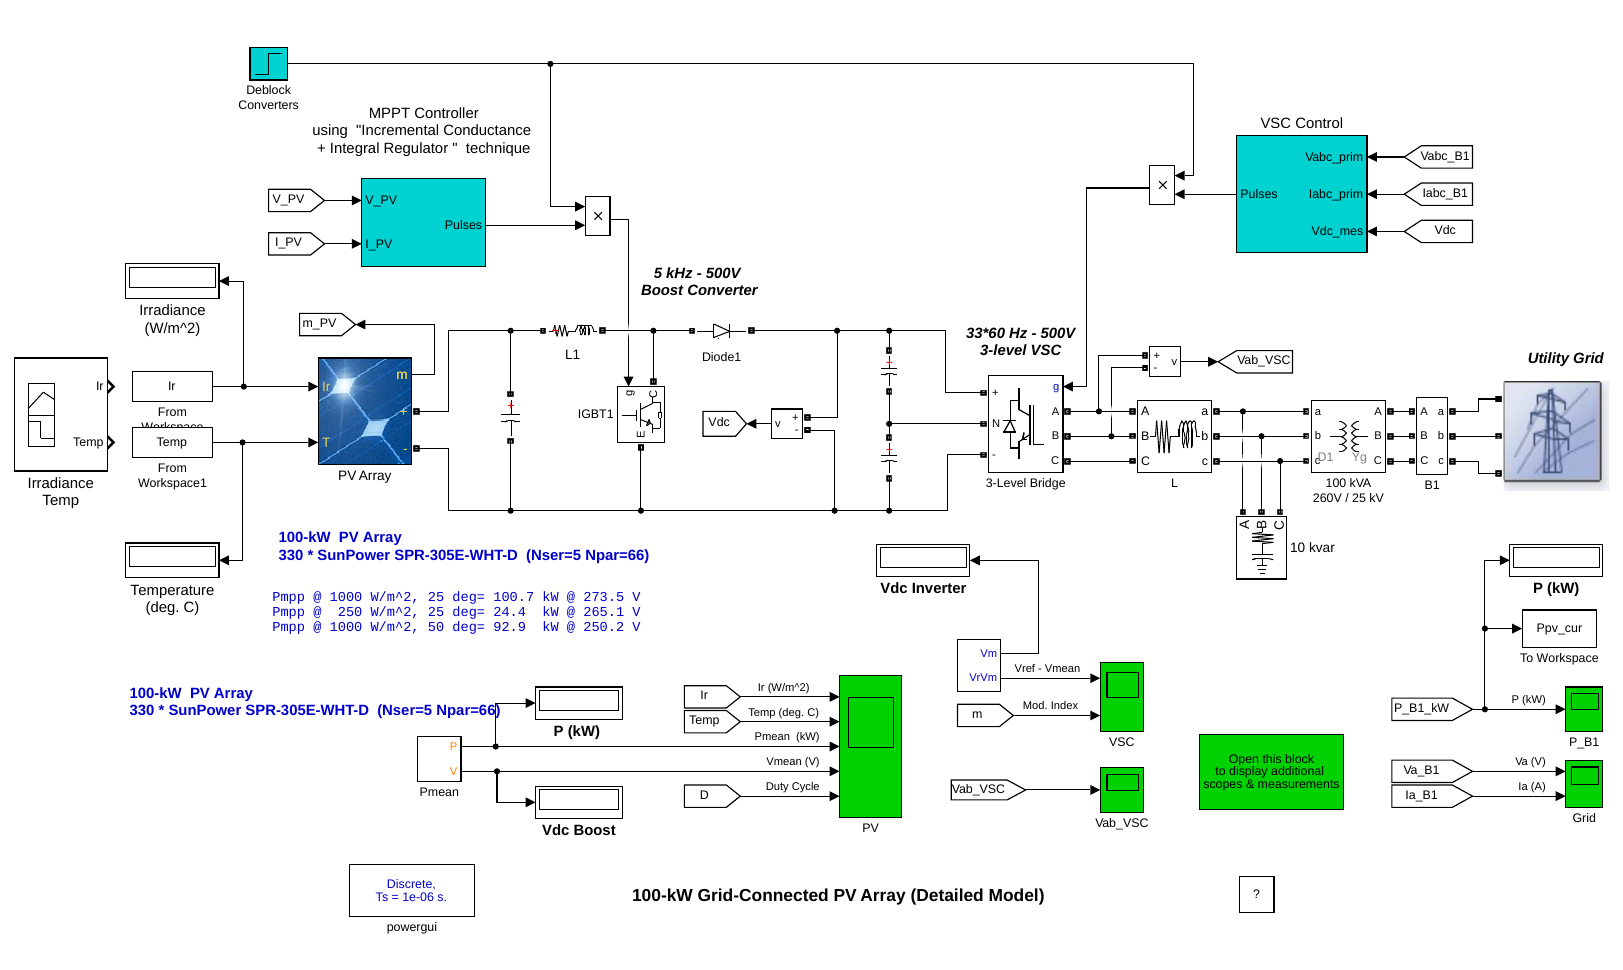
\includegraphics[width=\textwidth]{Ppv_diagram.png}
    \caption{Diagrama de la planta fotovoltaica de 100kW conectada a una red}
    \label{fig:Ppv_diagram}
\end{figure}


El modelo simula una planta fotovoltaica con las siguientes características:
\begin{itemize}
    \item 100kW a 1000$W/m^2$
    \item Conectada a una red de 25kV de tres fases
    \item Conexión DC-DC con amplificador de tensión
    \item 1980-Hz con VSC de 3-niveles y 3-fases
    \item Condensador de 10kvar para el filtrado
\end{itemize}

Para llevar a cabo la simulación es necesario introducir las variables mas relevantes para el panel fotovoltaico: Radiación y Temperatura. Tiene como resultado la potencia instantanea en watios. El modelo evalua las entradas 1000 veces por segundo dando como resultado una detallada grafica de potencia producida.

La importación y exportación de los valores se ha realizado desde el workspace, donde se pre y post procesan las señales resultantes: Las entradas (Radiación y Temperatura) se formatean de acuerdo a las entradas del modelo y las salidas (La potencia) se discretiza a valor por hora, ya que se evalua la potencia a un ratio de 1000 veces por 1 segundo de simulación.

La quicena de potencia que usaremos es la descrita entre el 1 y el 16 de abril. Se puede observar en la gráfica \ref{fig:Ppv_output} donde el eje x son los dias y el y la potencia generada en watios.

El resultado de la simulación puede observarse en la siguiente figura:

\begin{figure}[h]
    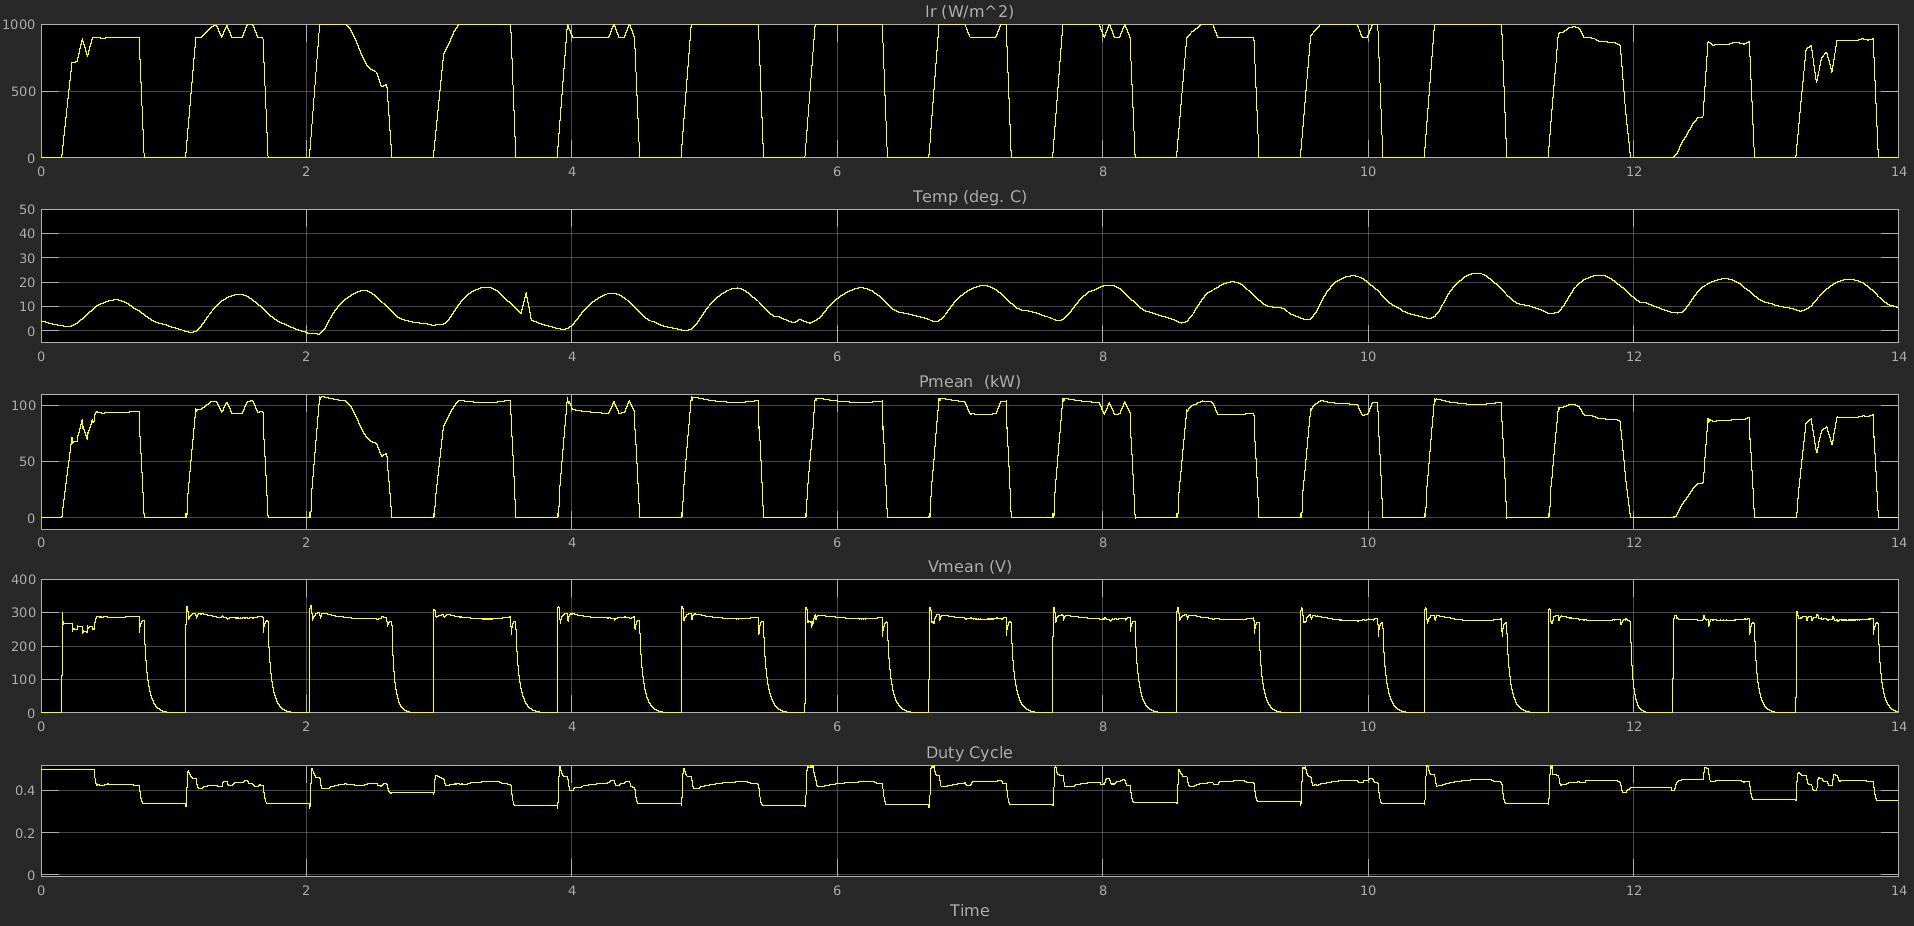
\includegraphics[width=\textwidth]{Model_cur_outputs_010417.jpg}
    \caption{Salida de la planta fotovoltaica}
    \label{fig:Ppv_output}
\end{figure}

\subsection{Modelos}
\label{sub:Modelos}

Para el estudio se han probado los siguientes modelos.

\begin{itemize}
    \item EWMA
    \item Predictor for adaptive management from ETHZ
    \item 2D linear predictor
    \item WCMA
    \item WCMA-PDR
    \item Neural network
    \item N4SID
\end{itemize}

Para la experimentación se ha usado el mismo periodo de 15 dias, entre el 15 y el 30 de marzo del 2017.

Los resultados mostrados a continuación se presentan como energía real producida más energía predicha y error entre ambas.


\subsubsection{EWMA}
\label{ssub:ewma}

En la gráfica se puede observar que usa los valores del dia anterior con una ligera atenuacion de la media de las predicciones pasadas. El nivel de error es alto durante el amanecer y el ocaso.

Horizonte de predicción: 24h
$\alpha = TODO$

\begin{figure}[h]
    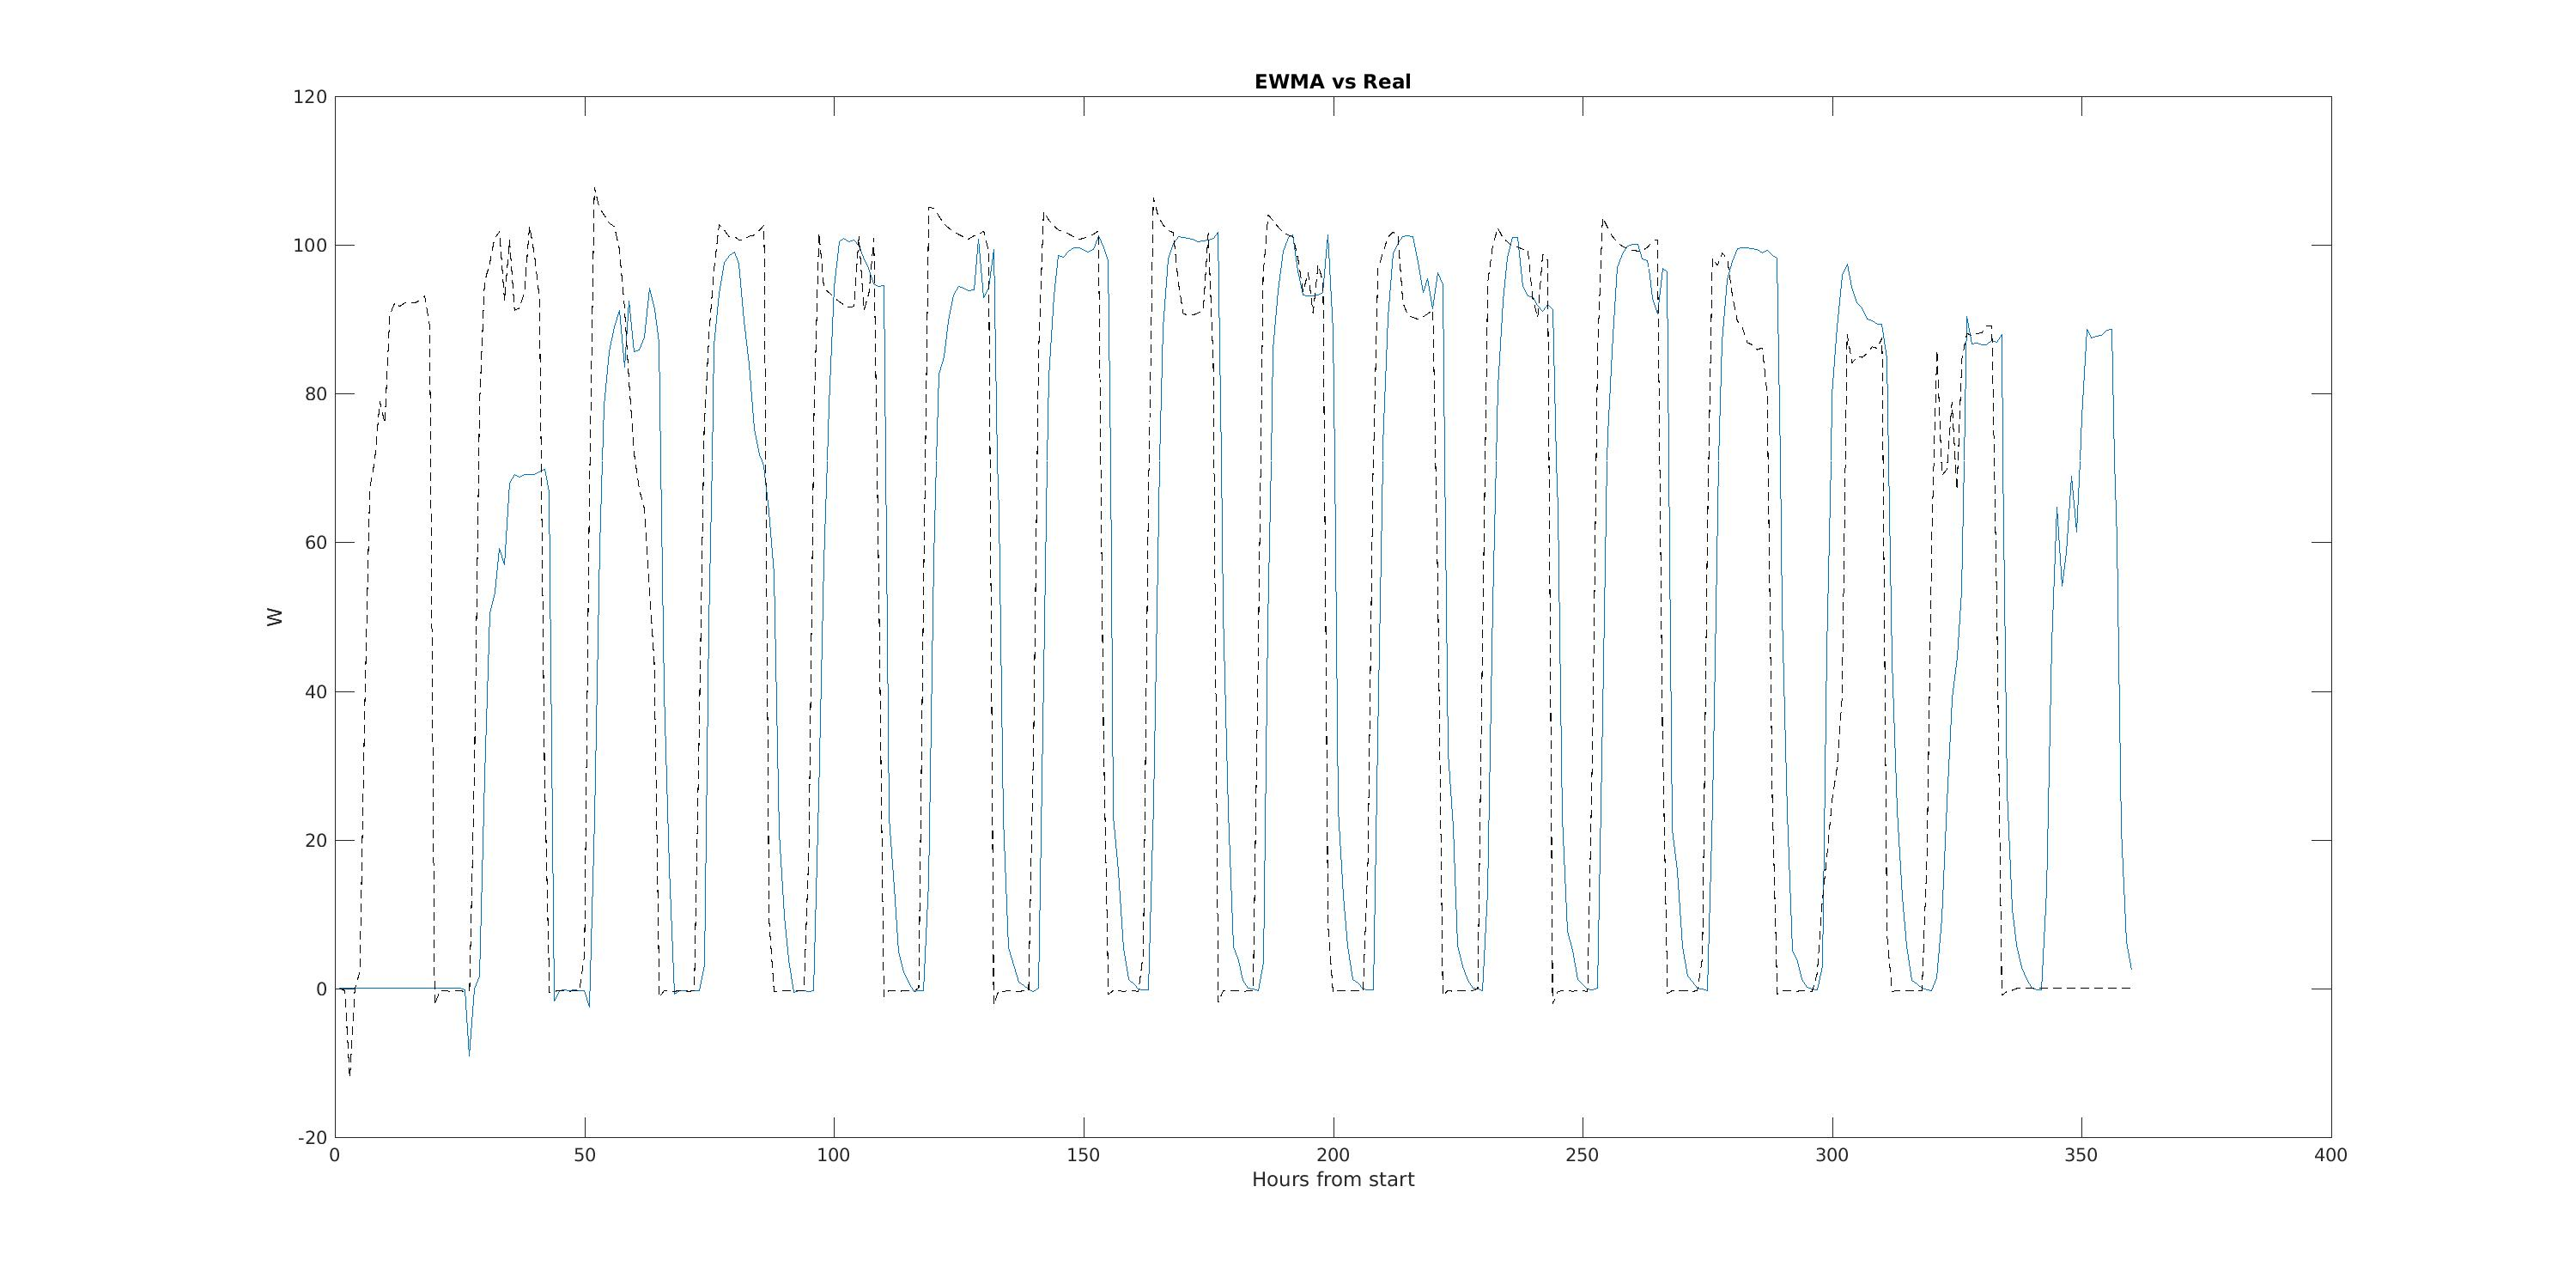
\includegraphics[width=\textwidth]{EWMA.jpg}
    \caption{EWMA Prediction accurancy}
    \label{fig:ewma_comp}
\end{figure}

\begin{figure}[h]
    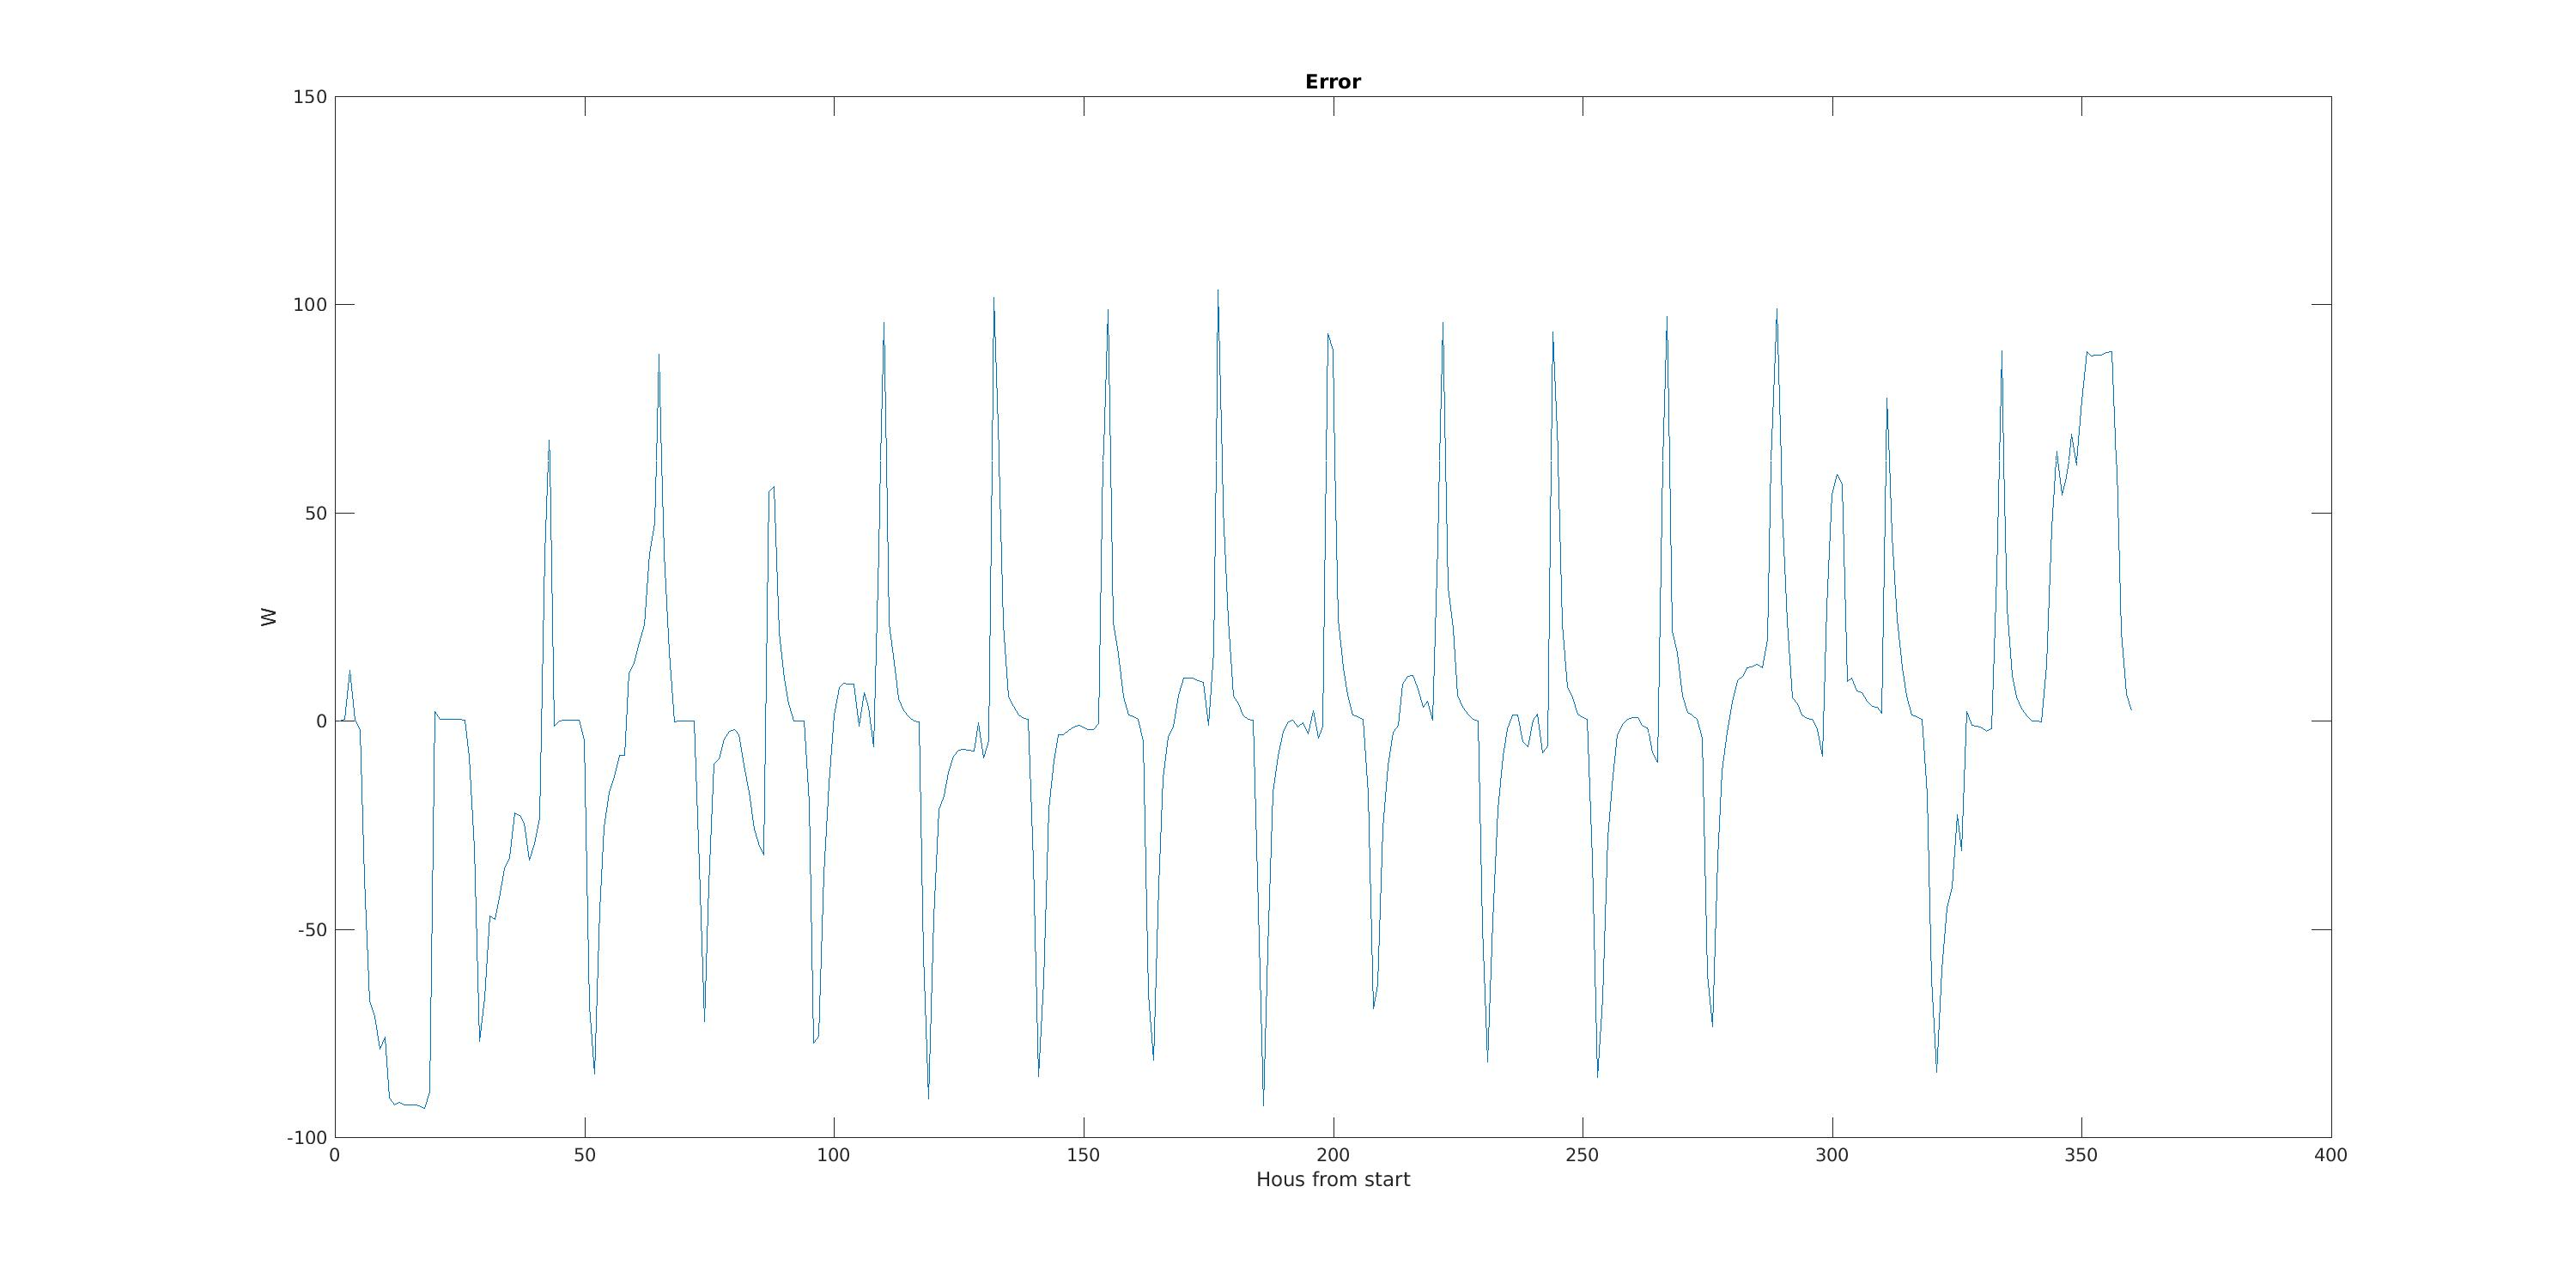
\includegraphics[width=\textwidth]{EWMA_error.jpg}
    \caption{EWMA Prediction error}
    \label{fig:ewma_error}
\end{figure}


\subsubsection{Adaptive power management (del ETHZ)}
 \label{ssub:adaptive_power_management}

El resultado de este tipo de predictor es muy similar al EWMA ya que realiza un cálculo basculado de el valor del dia anterior, pero sutilmente mejorado ya que tambien añade a la predicción los valores inmediatamente anteriores. El error en este caso es mas pronunciado en los extremos del dia pero mas estable en los puntos de irradiación estable.

Horizonte de predicción: 24h
$\alpha = TODO$

\begin{figure}[h]
    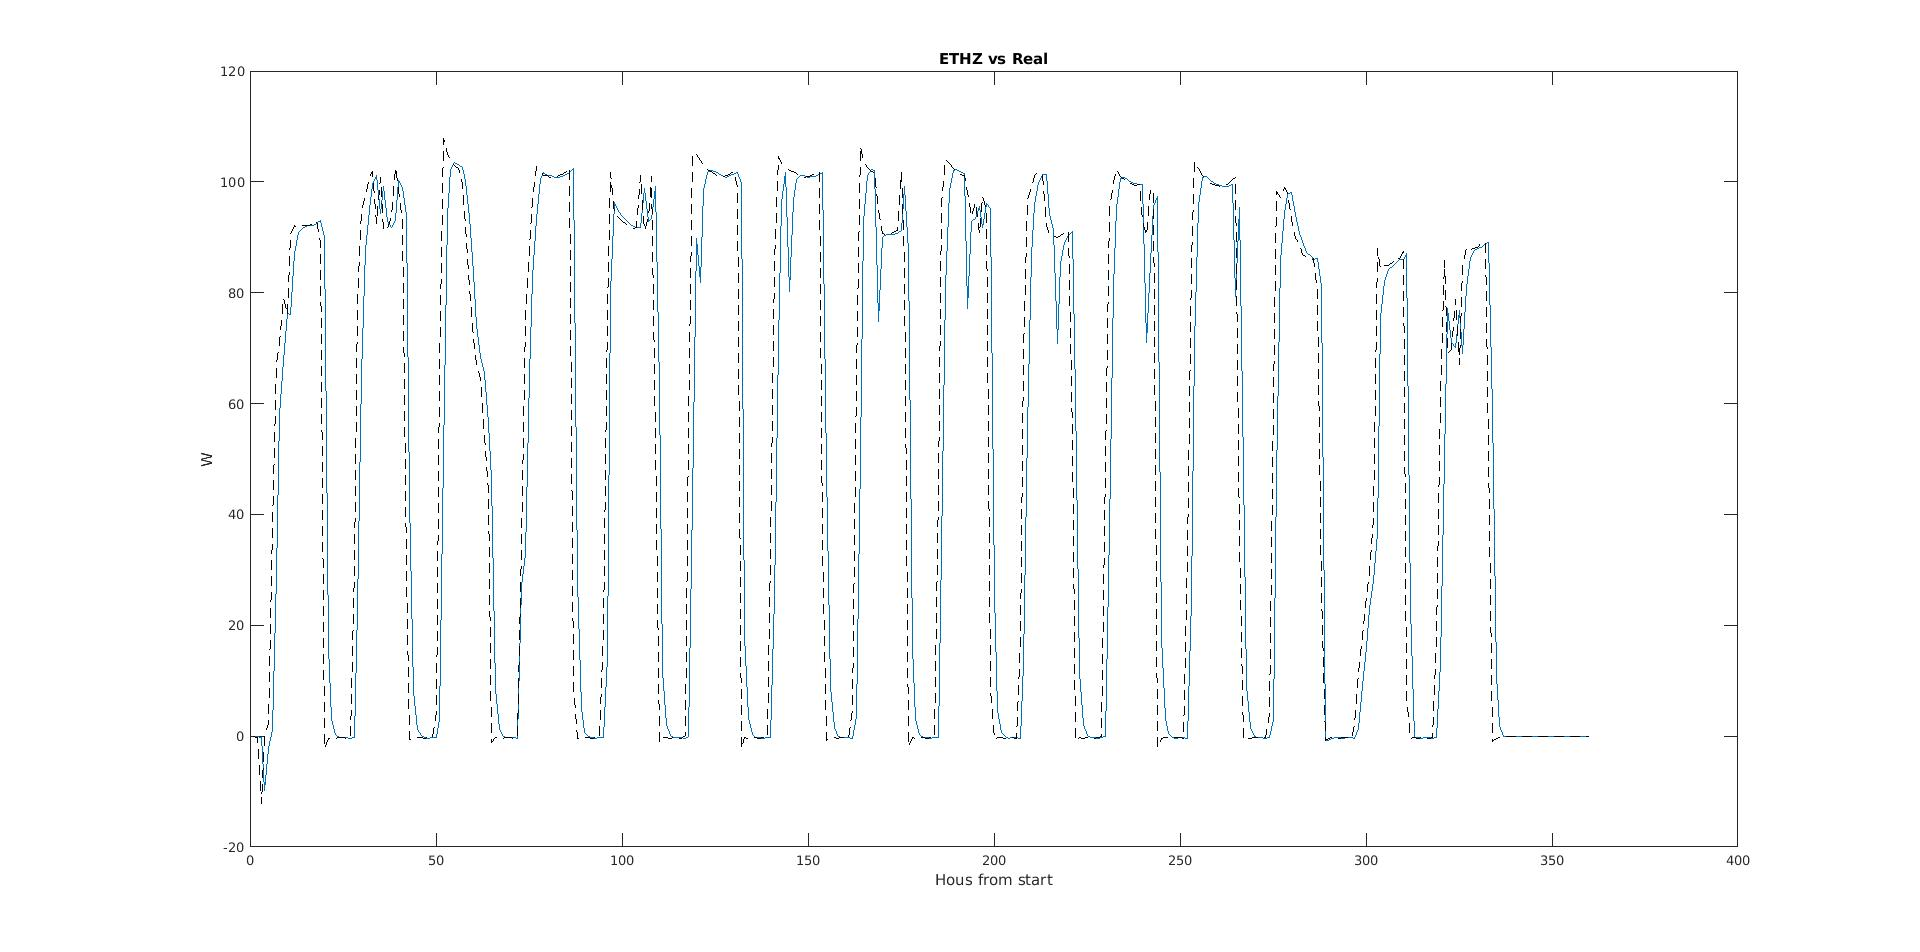
\includegraphics[width=\textwidth]{ETHZ.jpg}
    \caption{ETHZ Prediction accurancy}
    \label{fig:ethz_comp}
\end{figure}

\begin{figure}[h]
    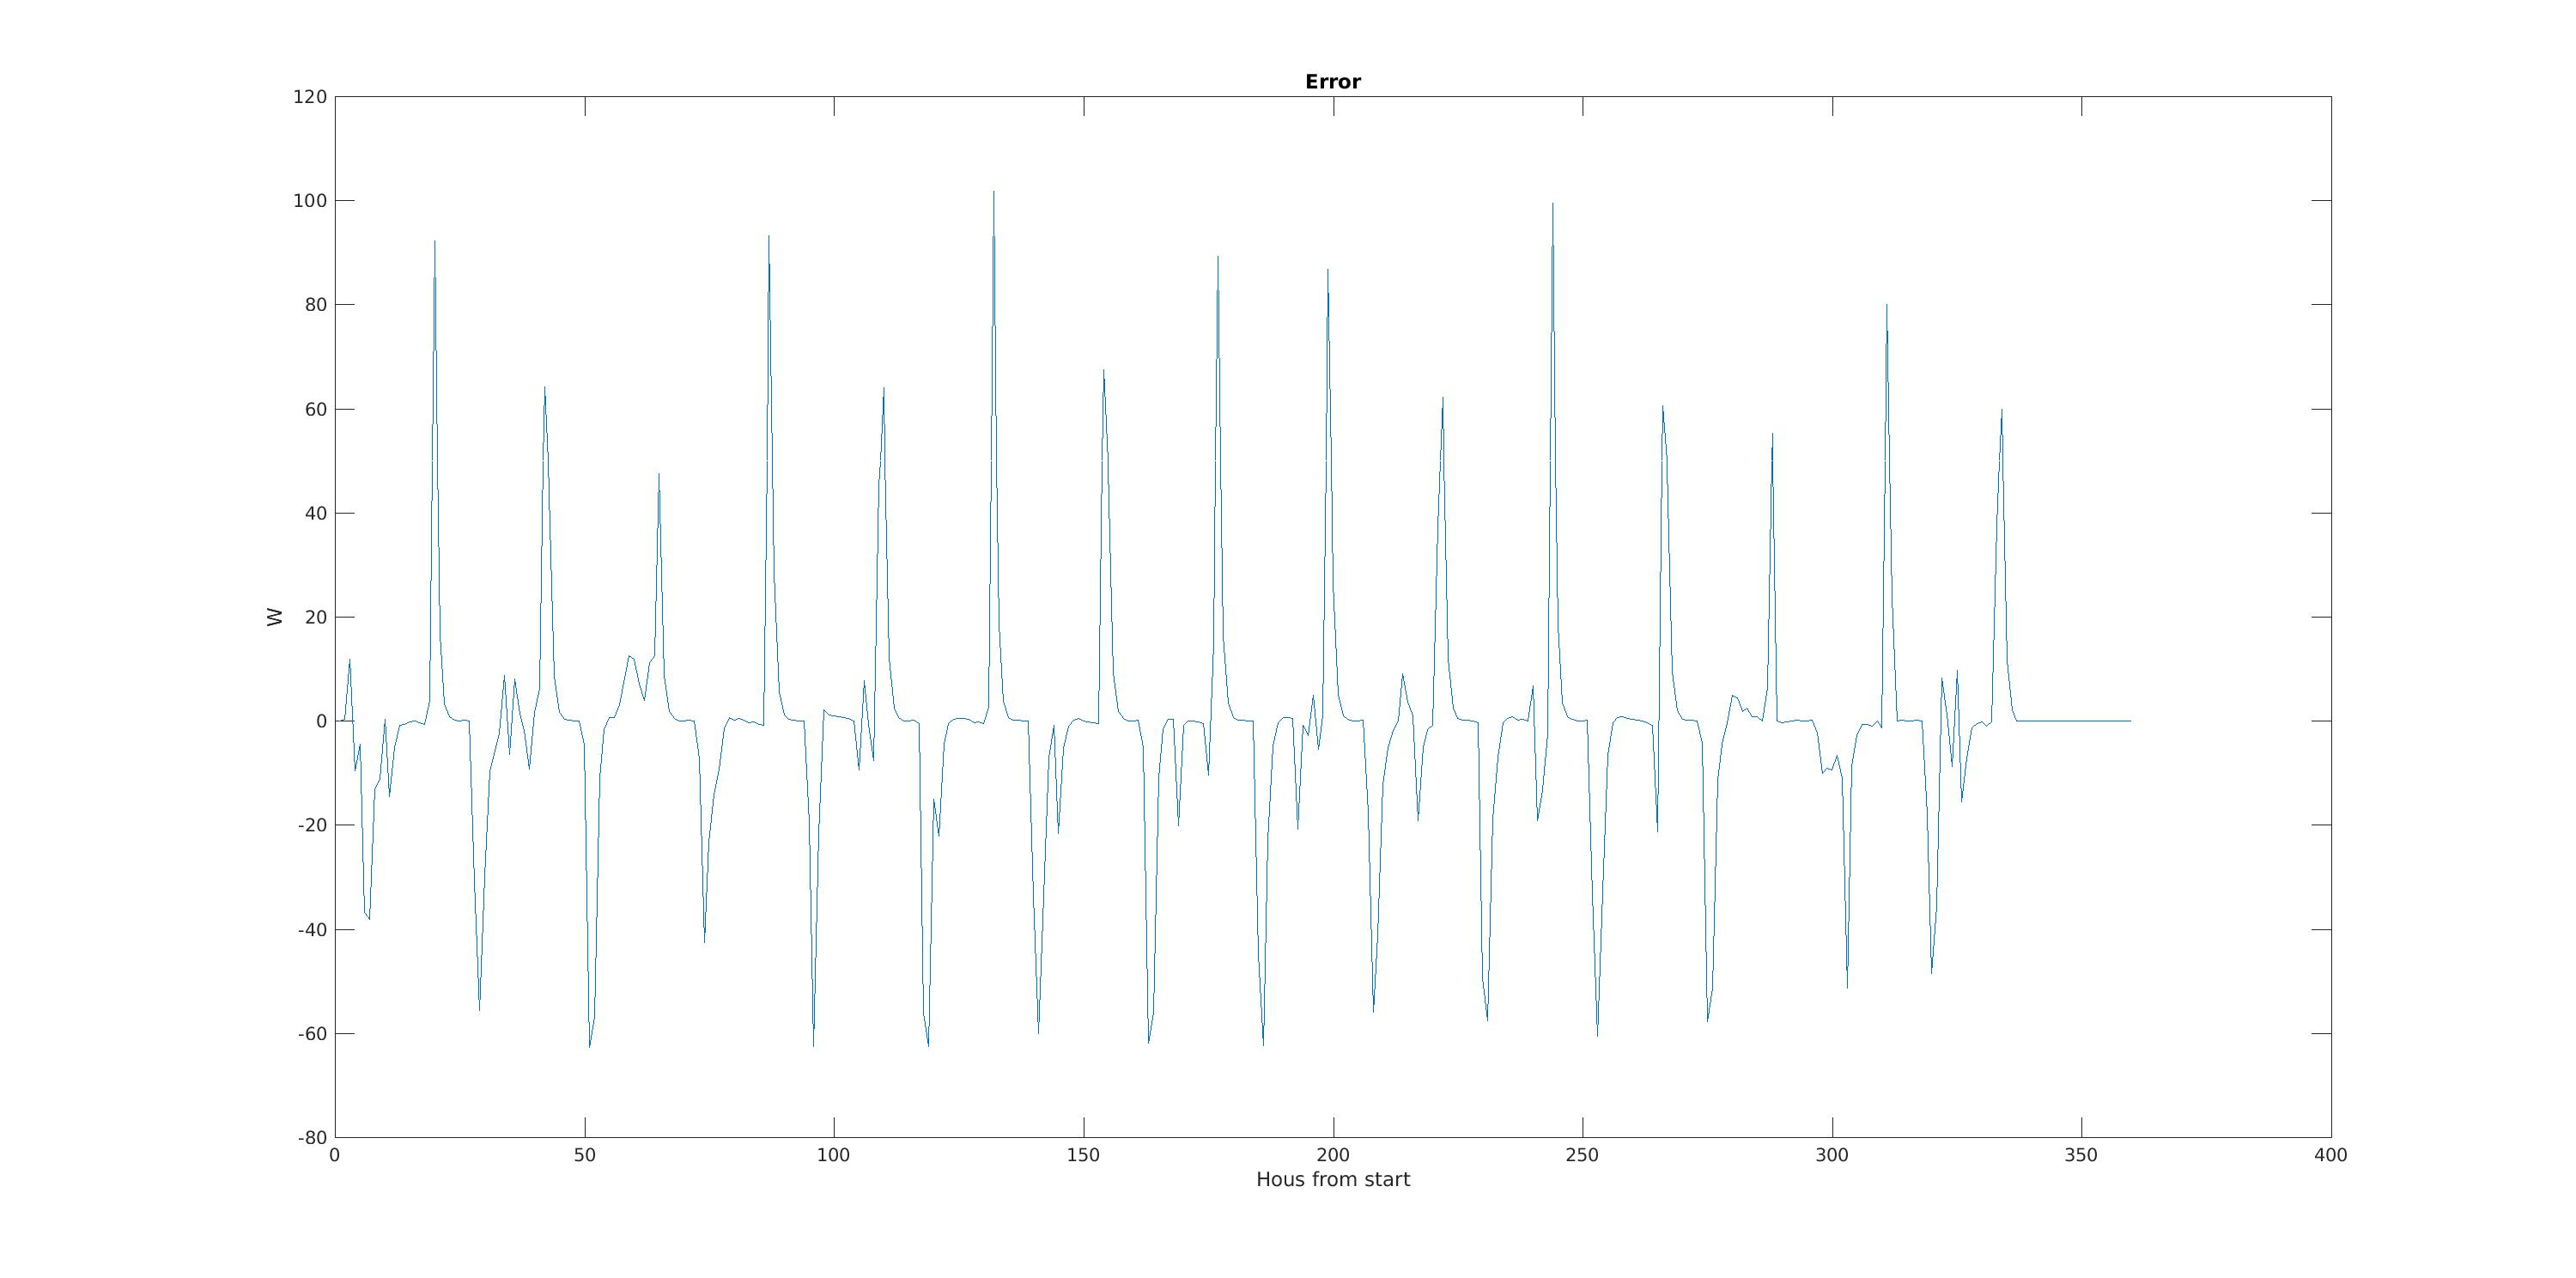
\includegraphics[width=\textwidth]{ETHZ_error.jpg}
    \caption{ETHZ Prediction error}
    \label{fig:ethz_error}
\end{figure}


\subsubsection{Optimal 2D prediction filter} 
\label{ssub:optimal_2d_prediction_filter}



\begin{figure}[h]
    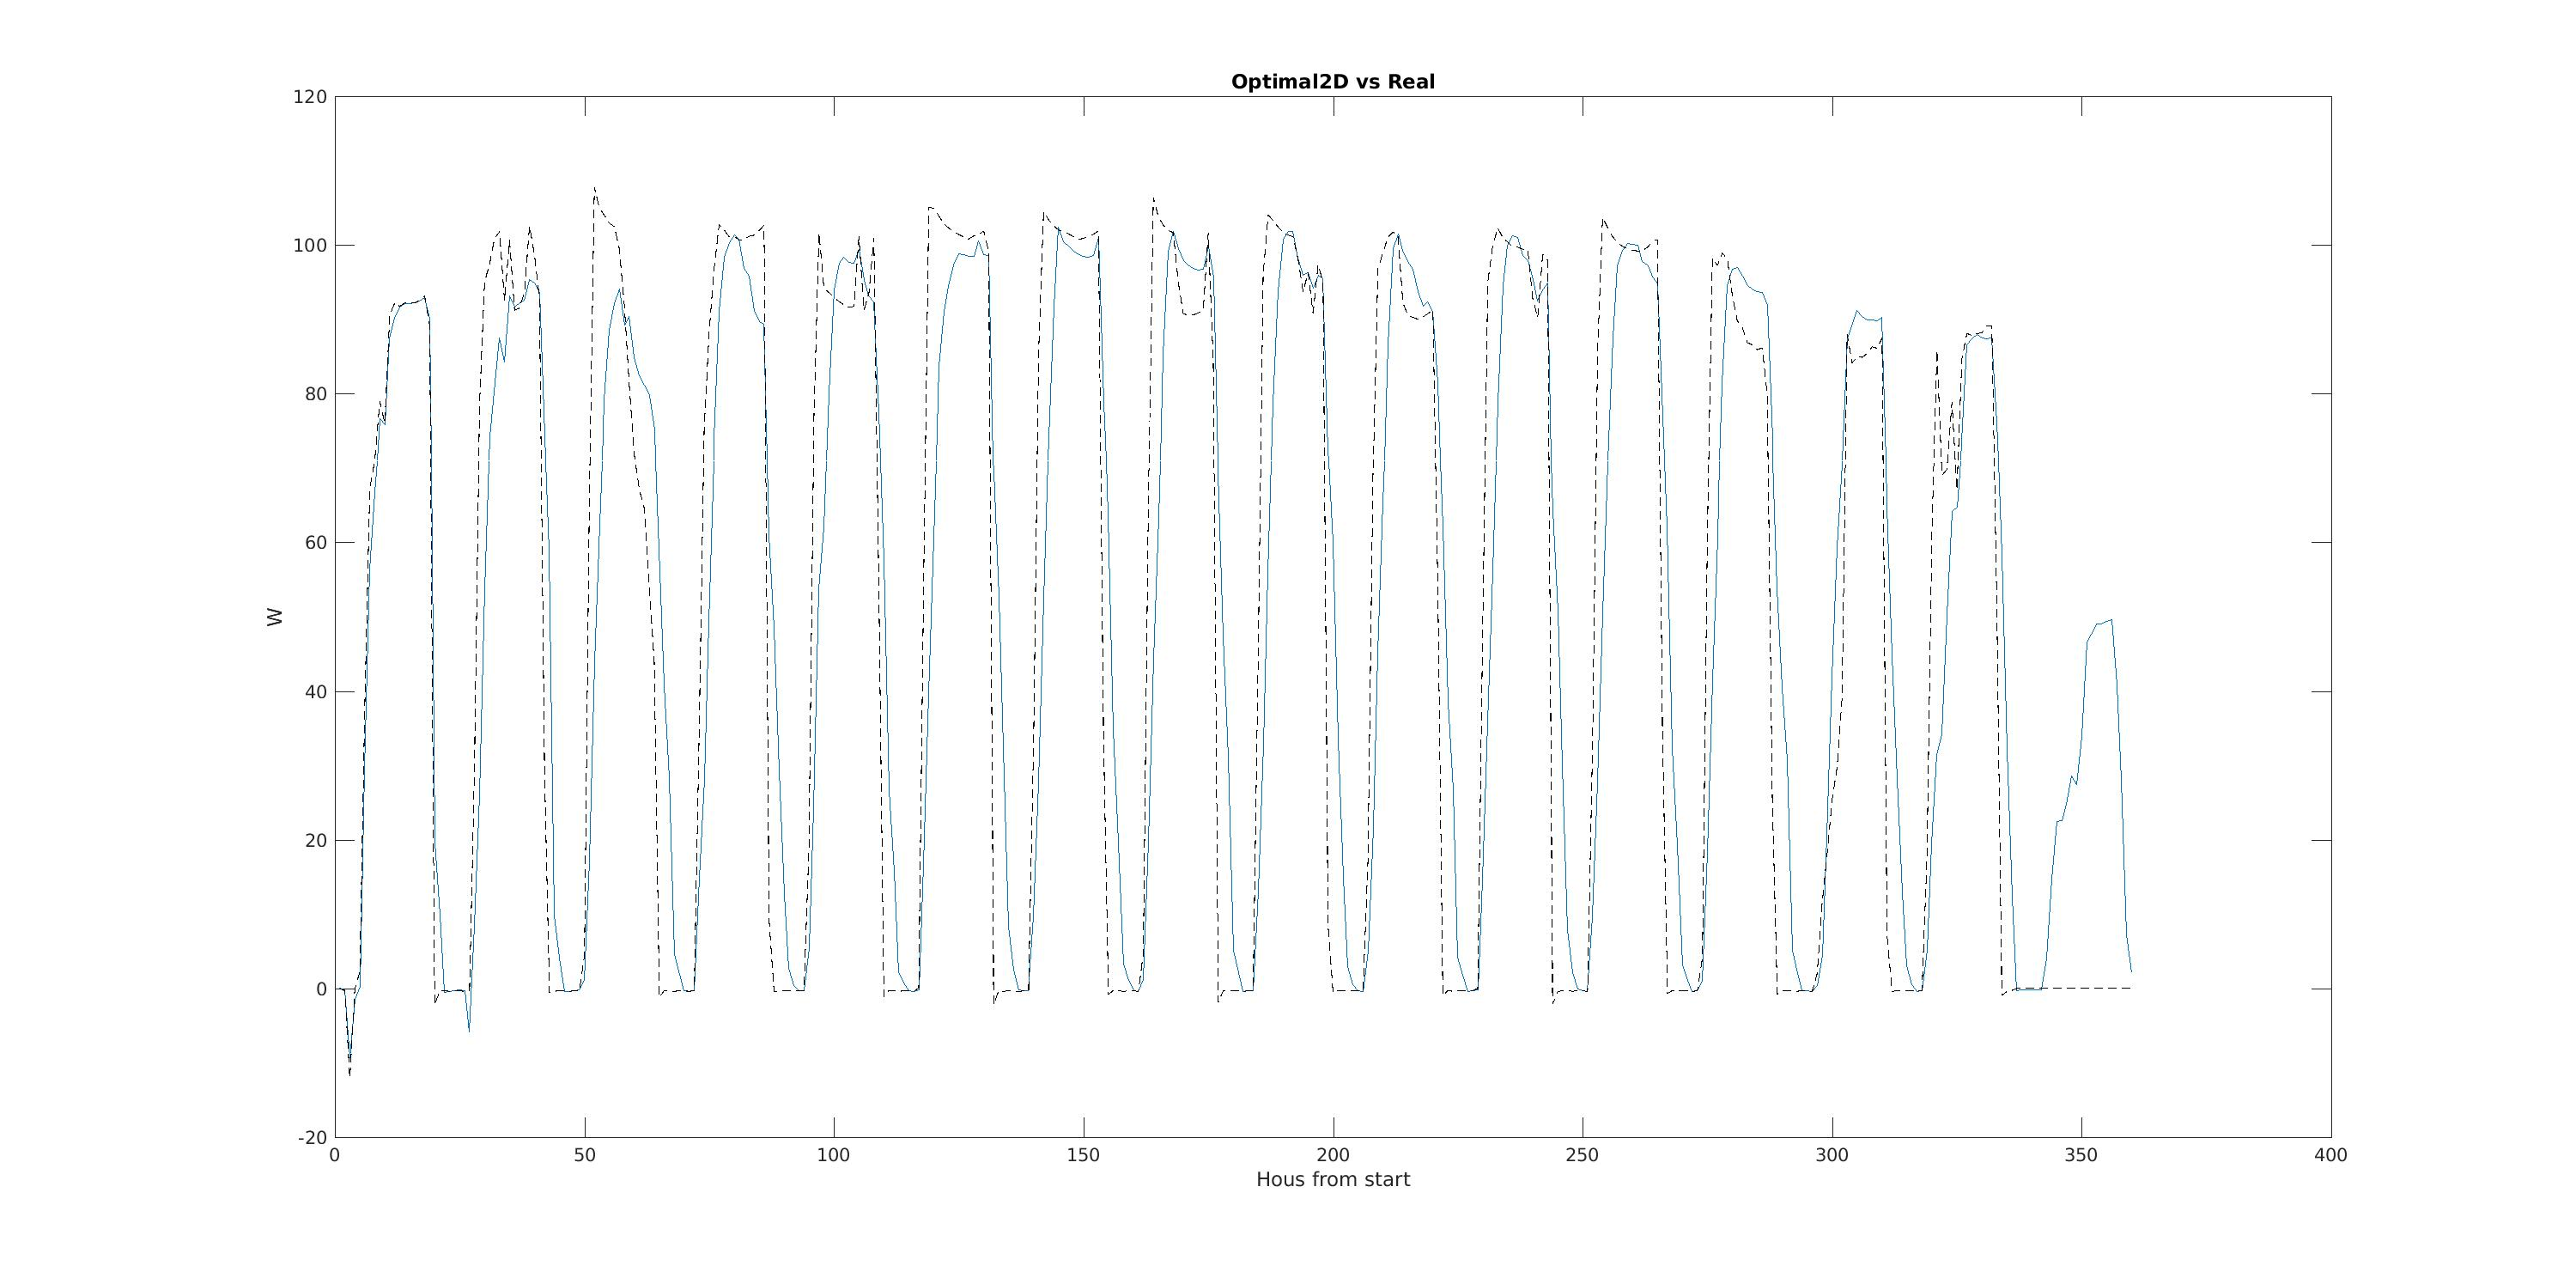
\includegraphics[width=\textwidth]{Optimal2D.jpg}
    \caption{2D filter Prediction accurancy}
    \label{fig:o2d_comp}
\end{figure}

\begin{figure}[h]
    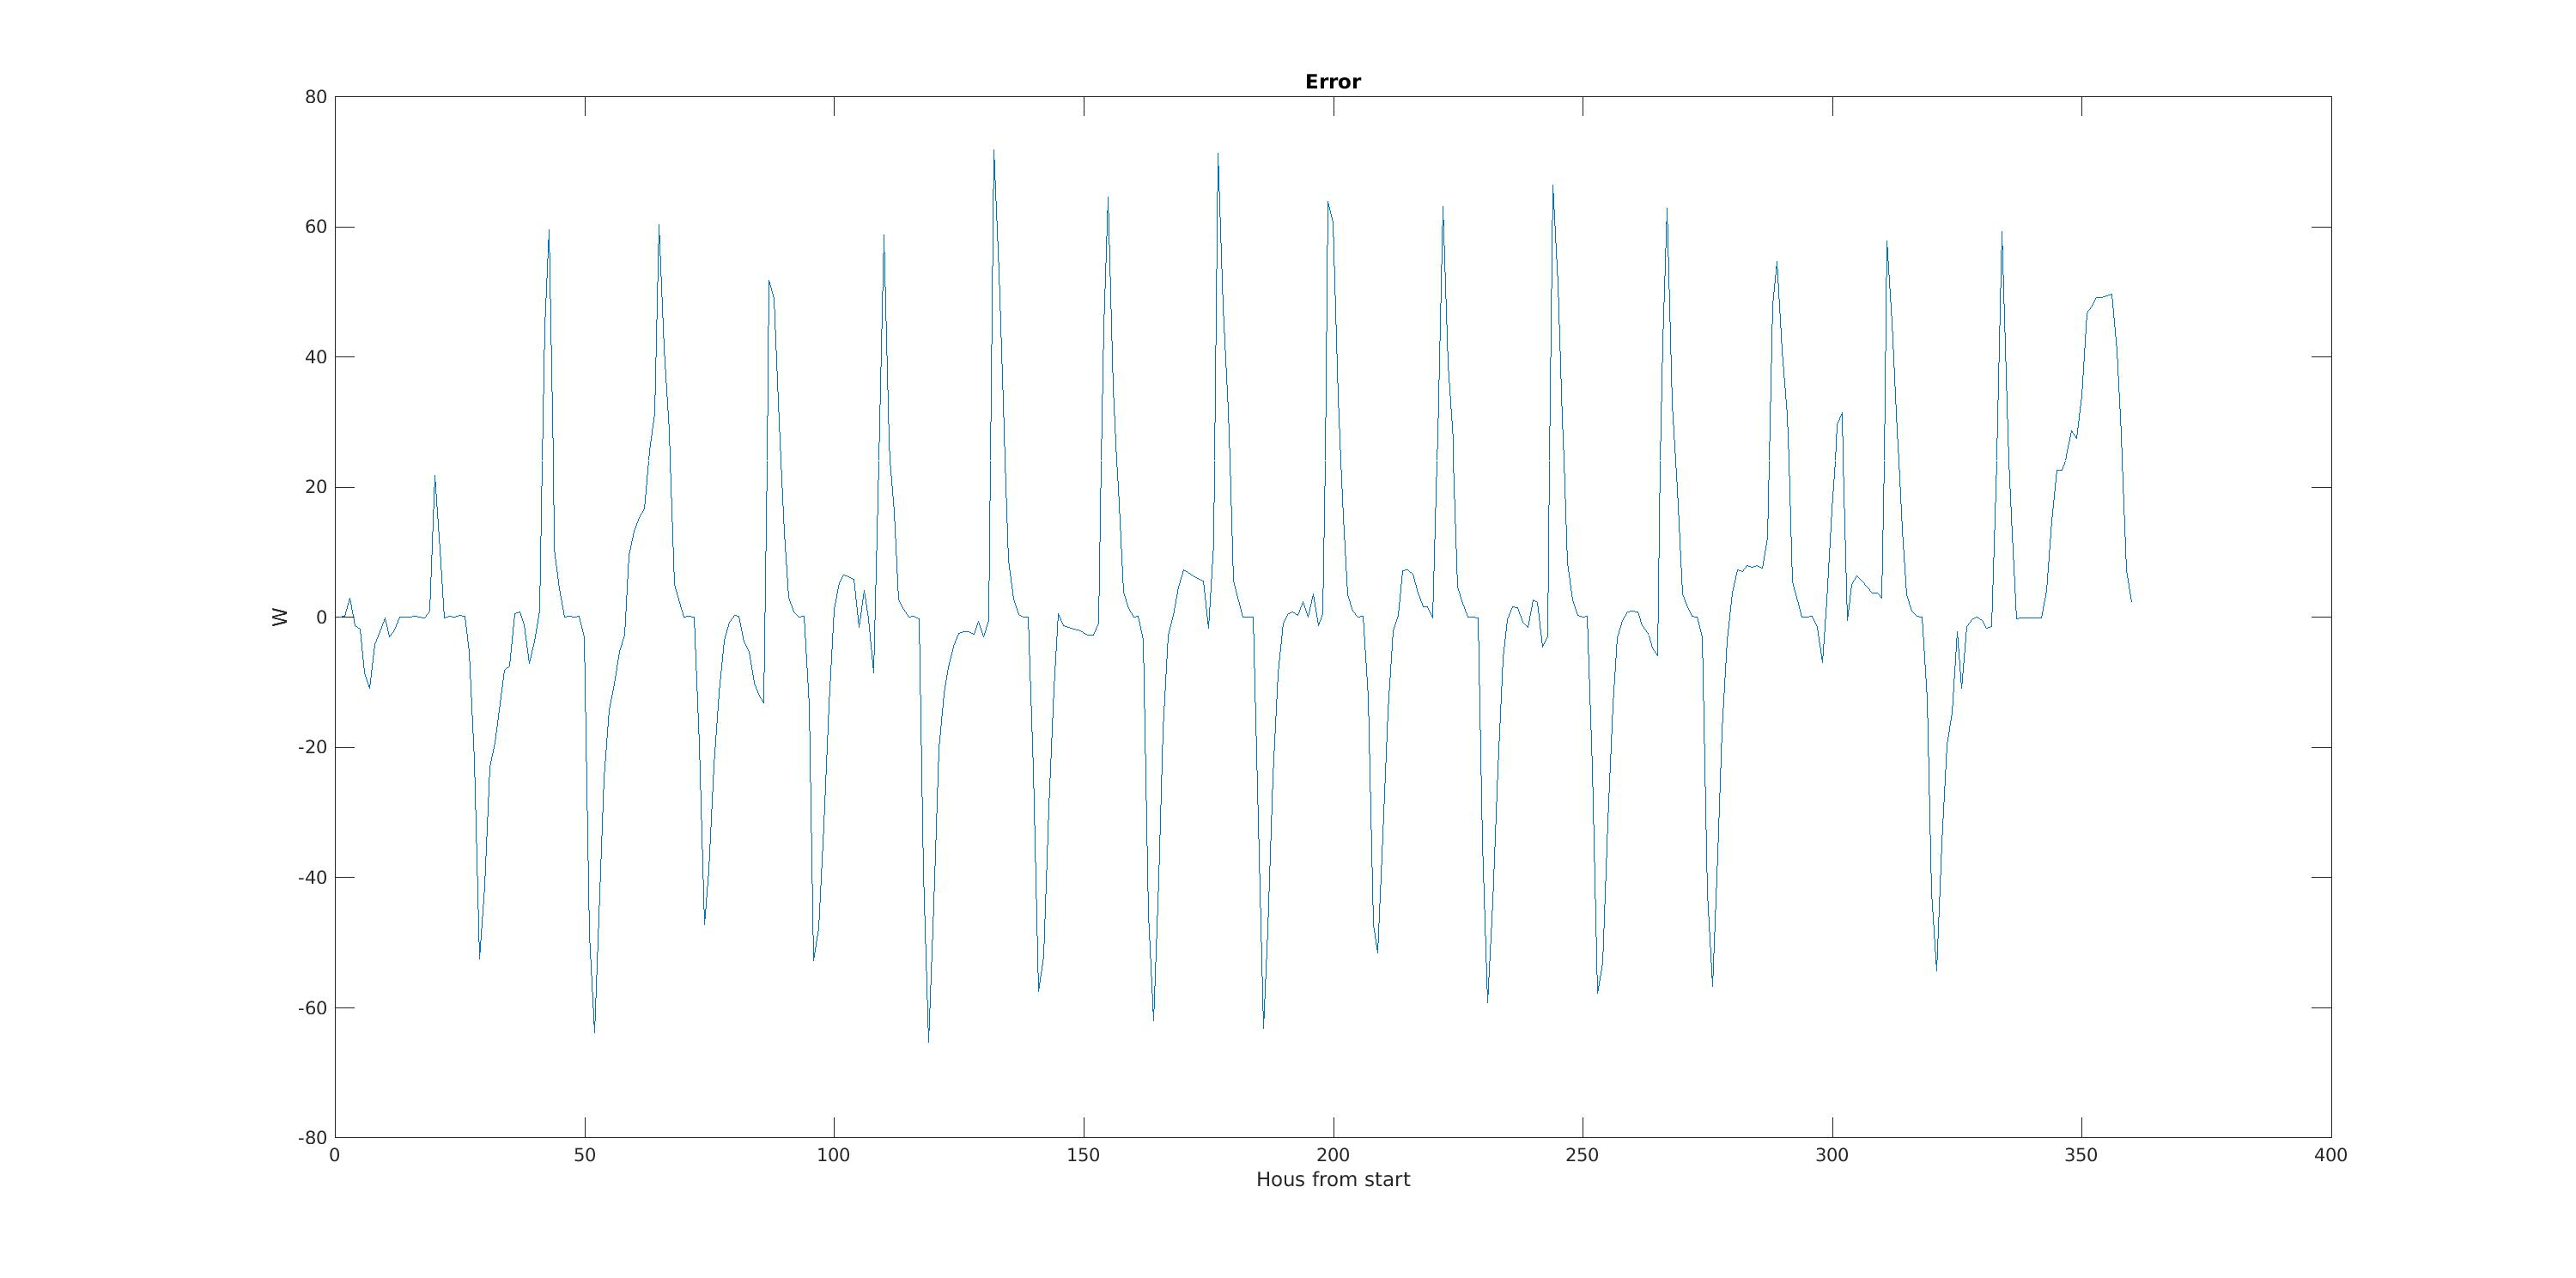
\includegraphics[width=\textwidth]{Optimal2D_error.jpg}
    \caption{2D filter Prediction error}
    \label{fig:o2d_error}
\end{figure}


\subsubsection{WCMA} 
\label{ssub:wcma}
\begin{figure}[h]
    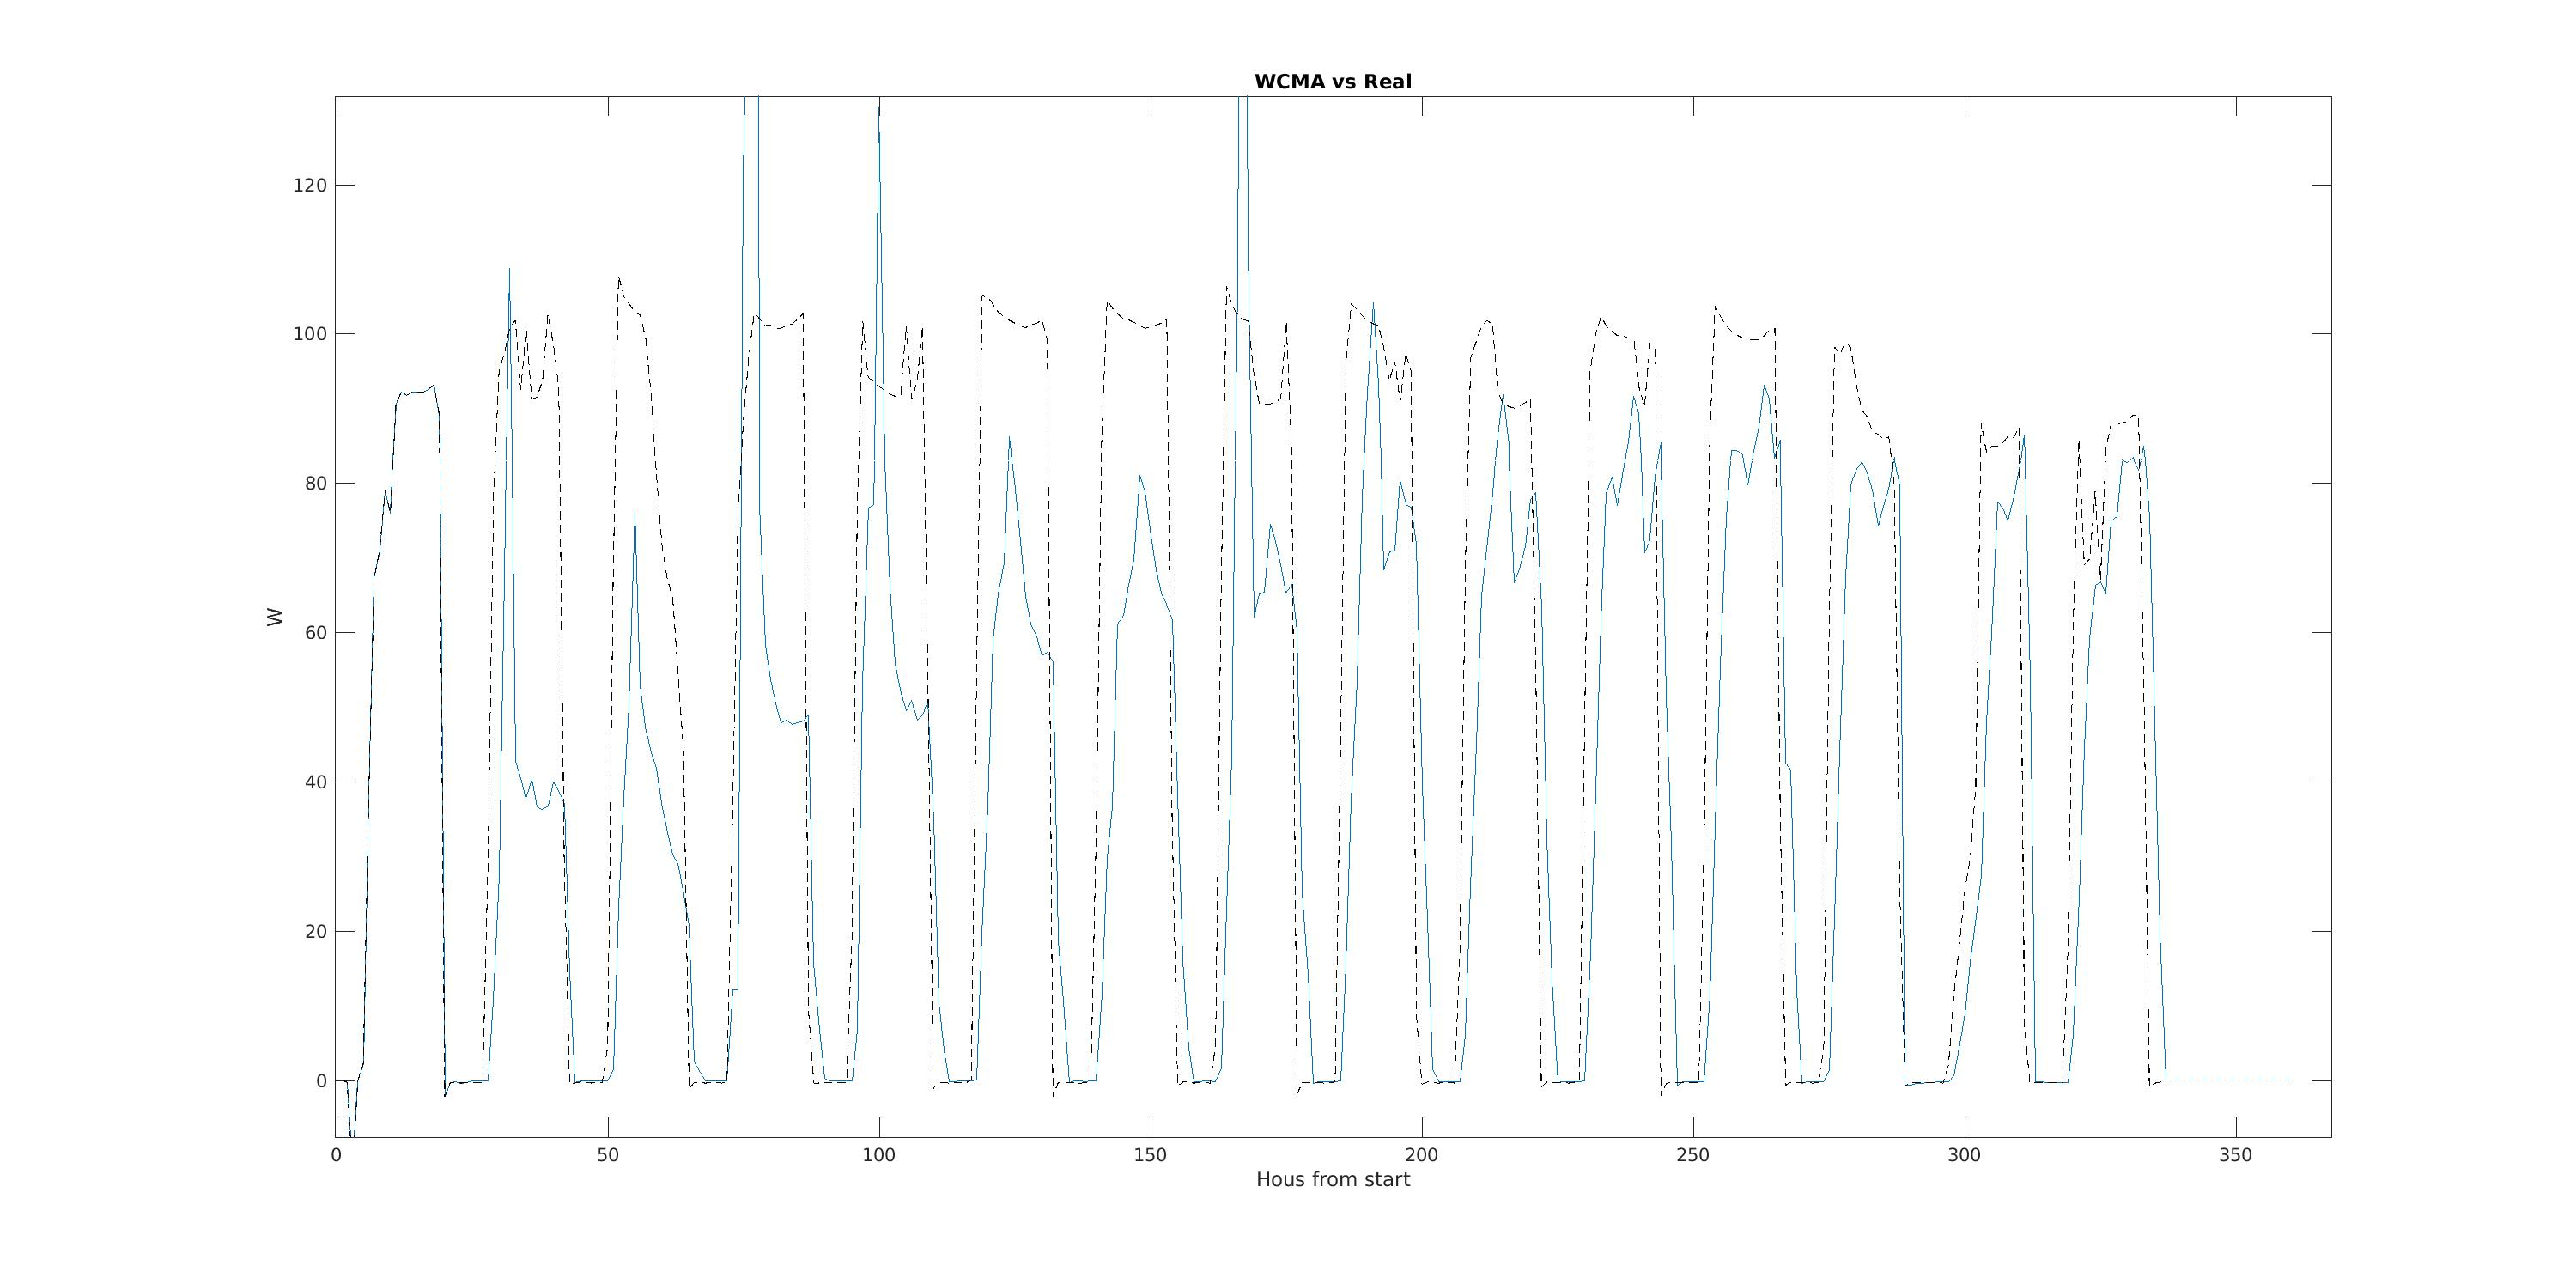
\includegraphics[width=\textwidth]{WCMA.jpg}
    \caption{WCMA Prediction accurancy}
    \label{fig:wcma_comp}
\end{figure}

\begin{figure}[h]
    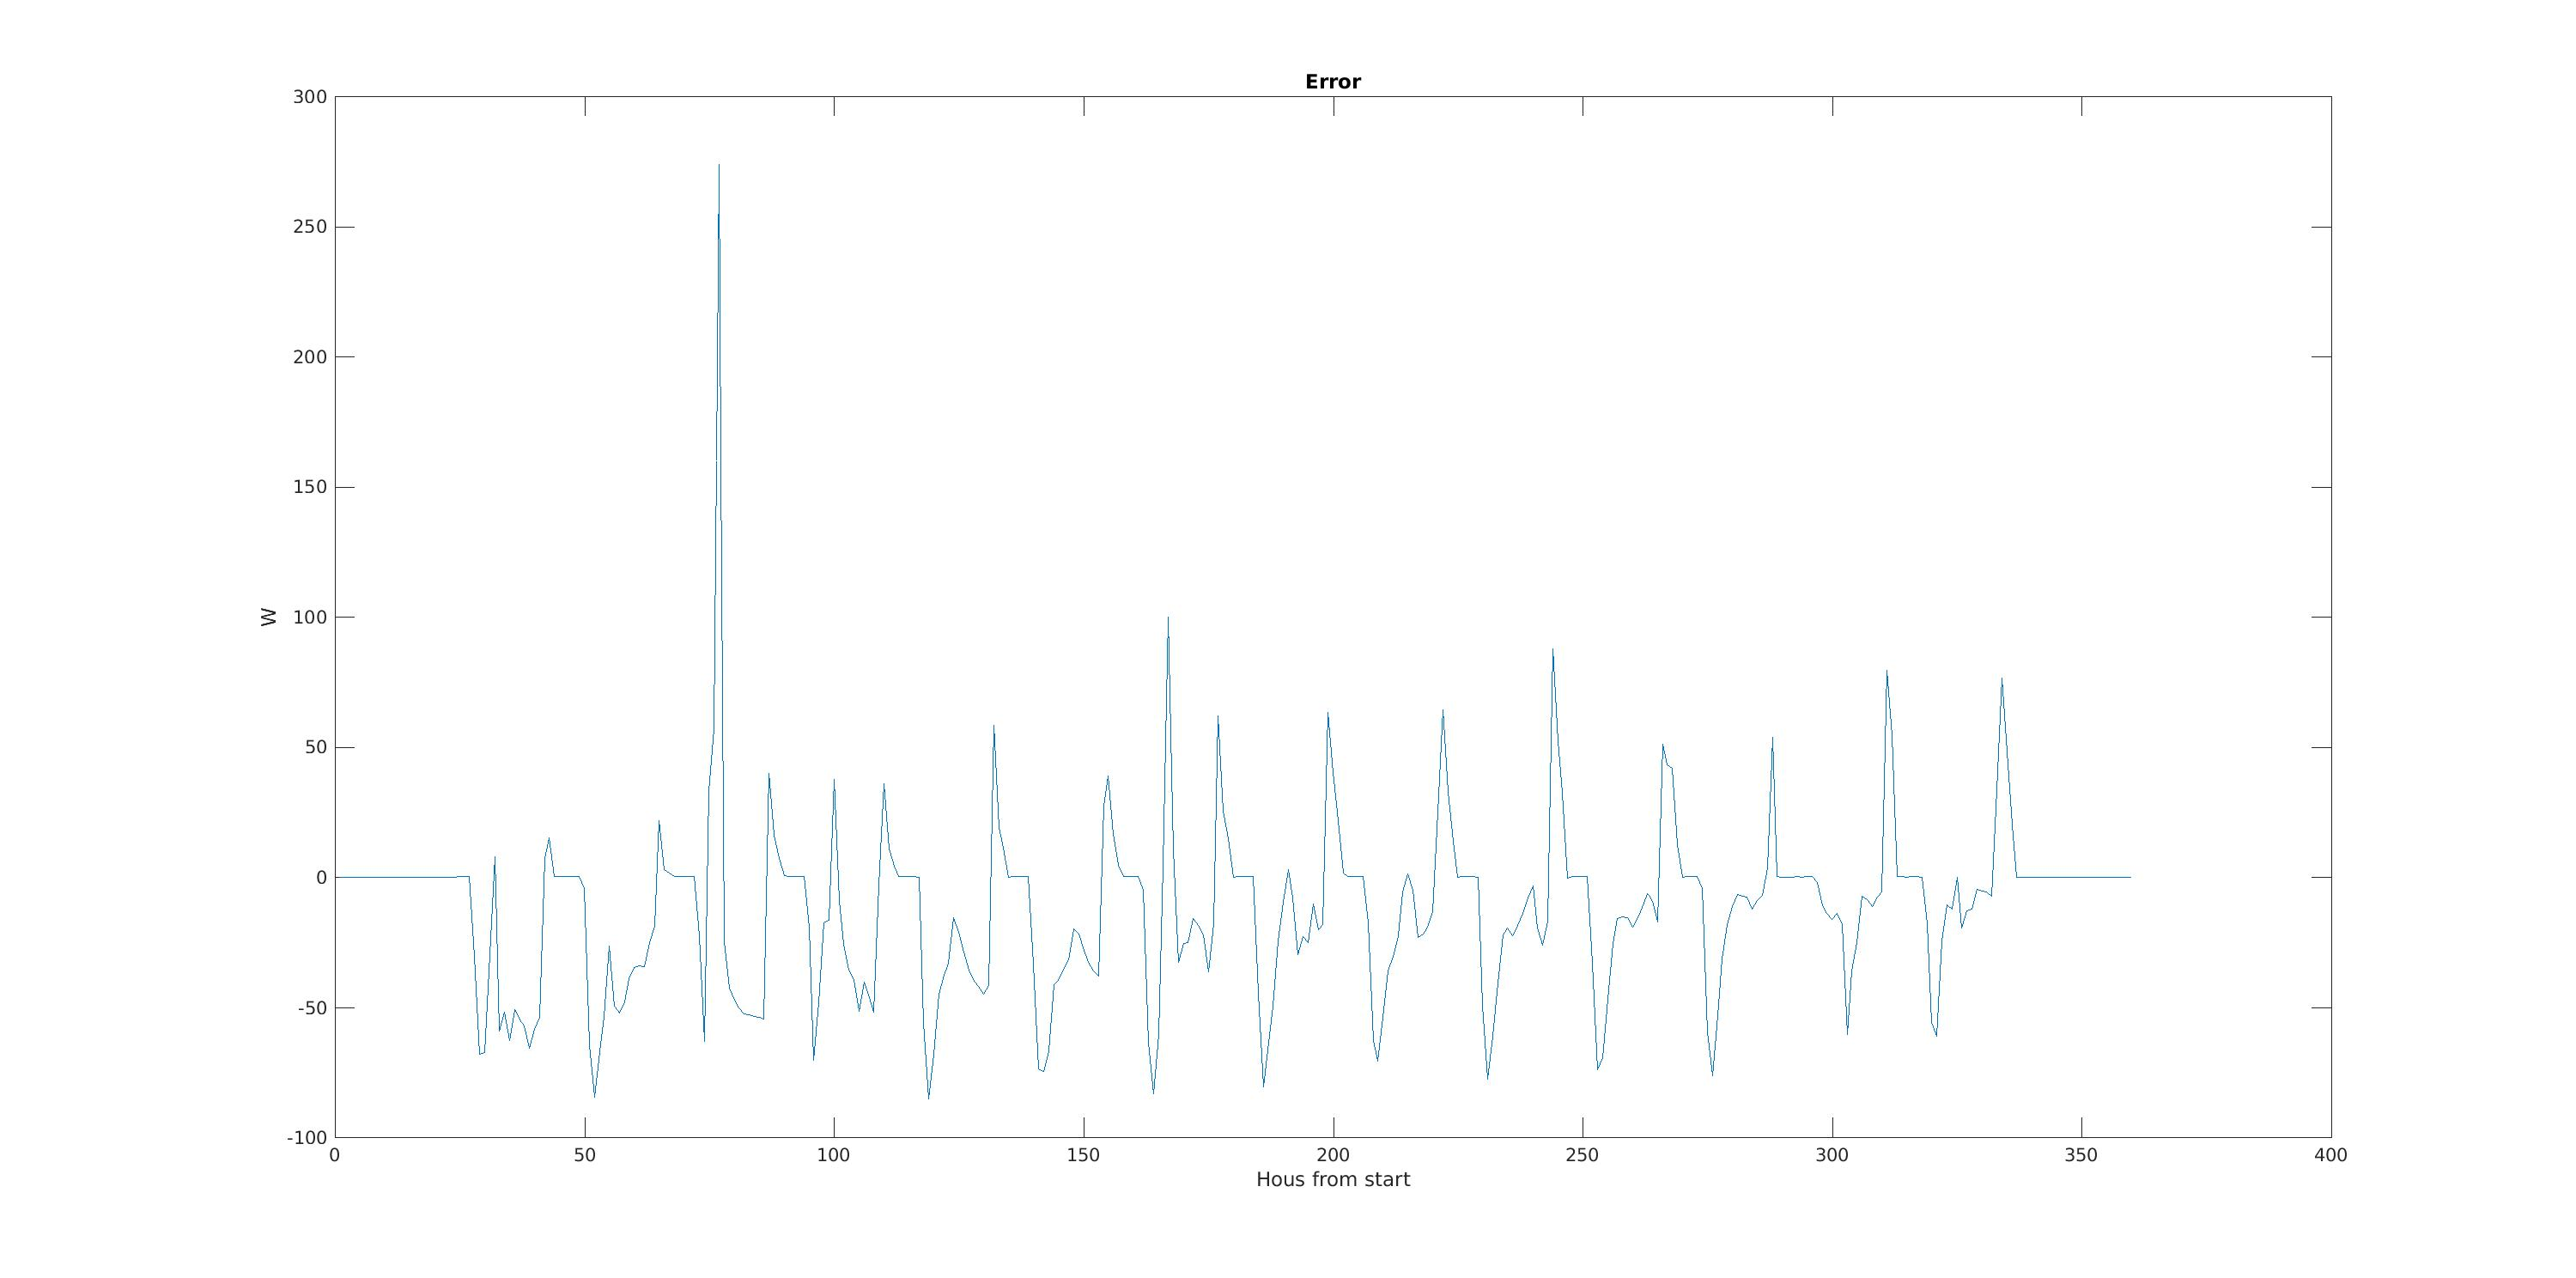
\includegraphics[width=\textwidth]{WCMA_error.jpg}
    \caption{WCMA Prediction error}
    \label{fig:wcma_error}
\end{figure}


\subsubsection{WCMA with PDR} 
\label{ssub:wcma_with_pdr}
\begin{figure}[h]
    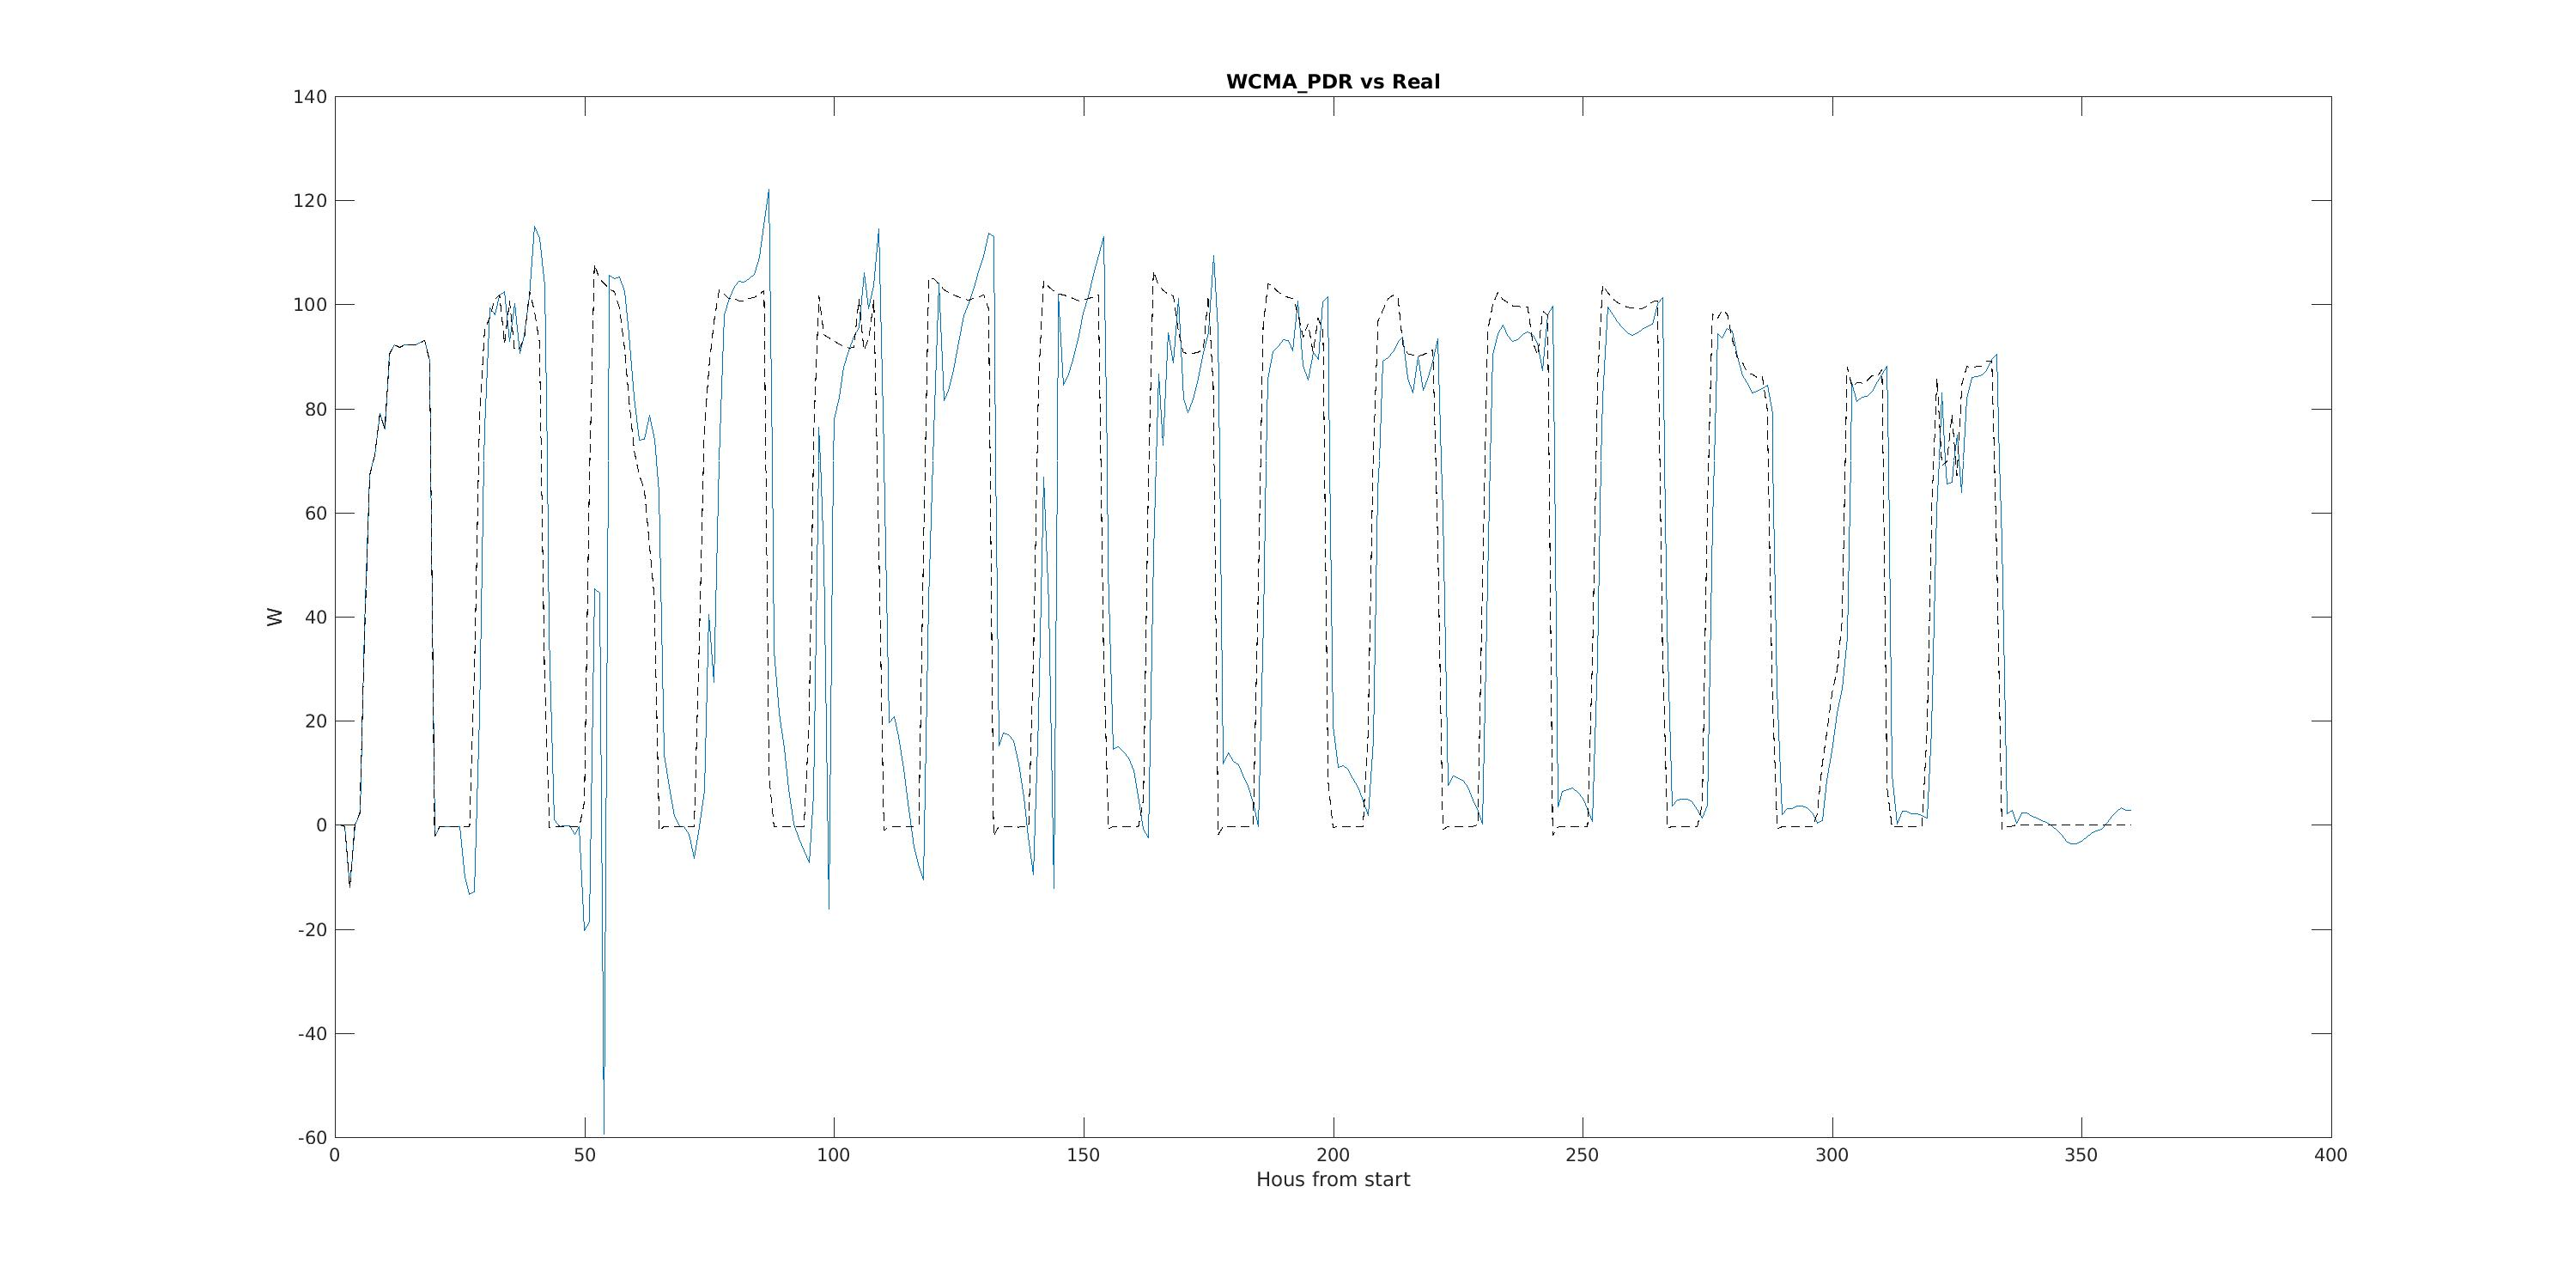
\includegraphics[width=\textwidth]{WCMA-PDR.jpg}
    \caption{WCMA with PDR Prediction accurancy}
    \label{fig:wcmapdr_comp}
\end{figure}

\begin{figure}[h]
    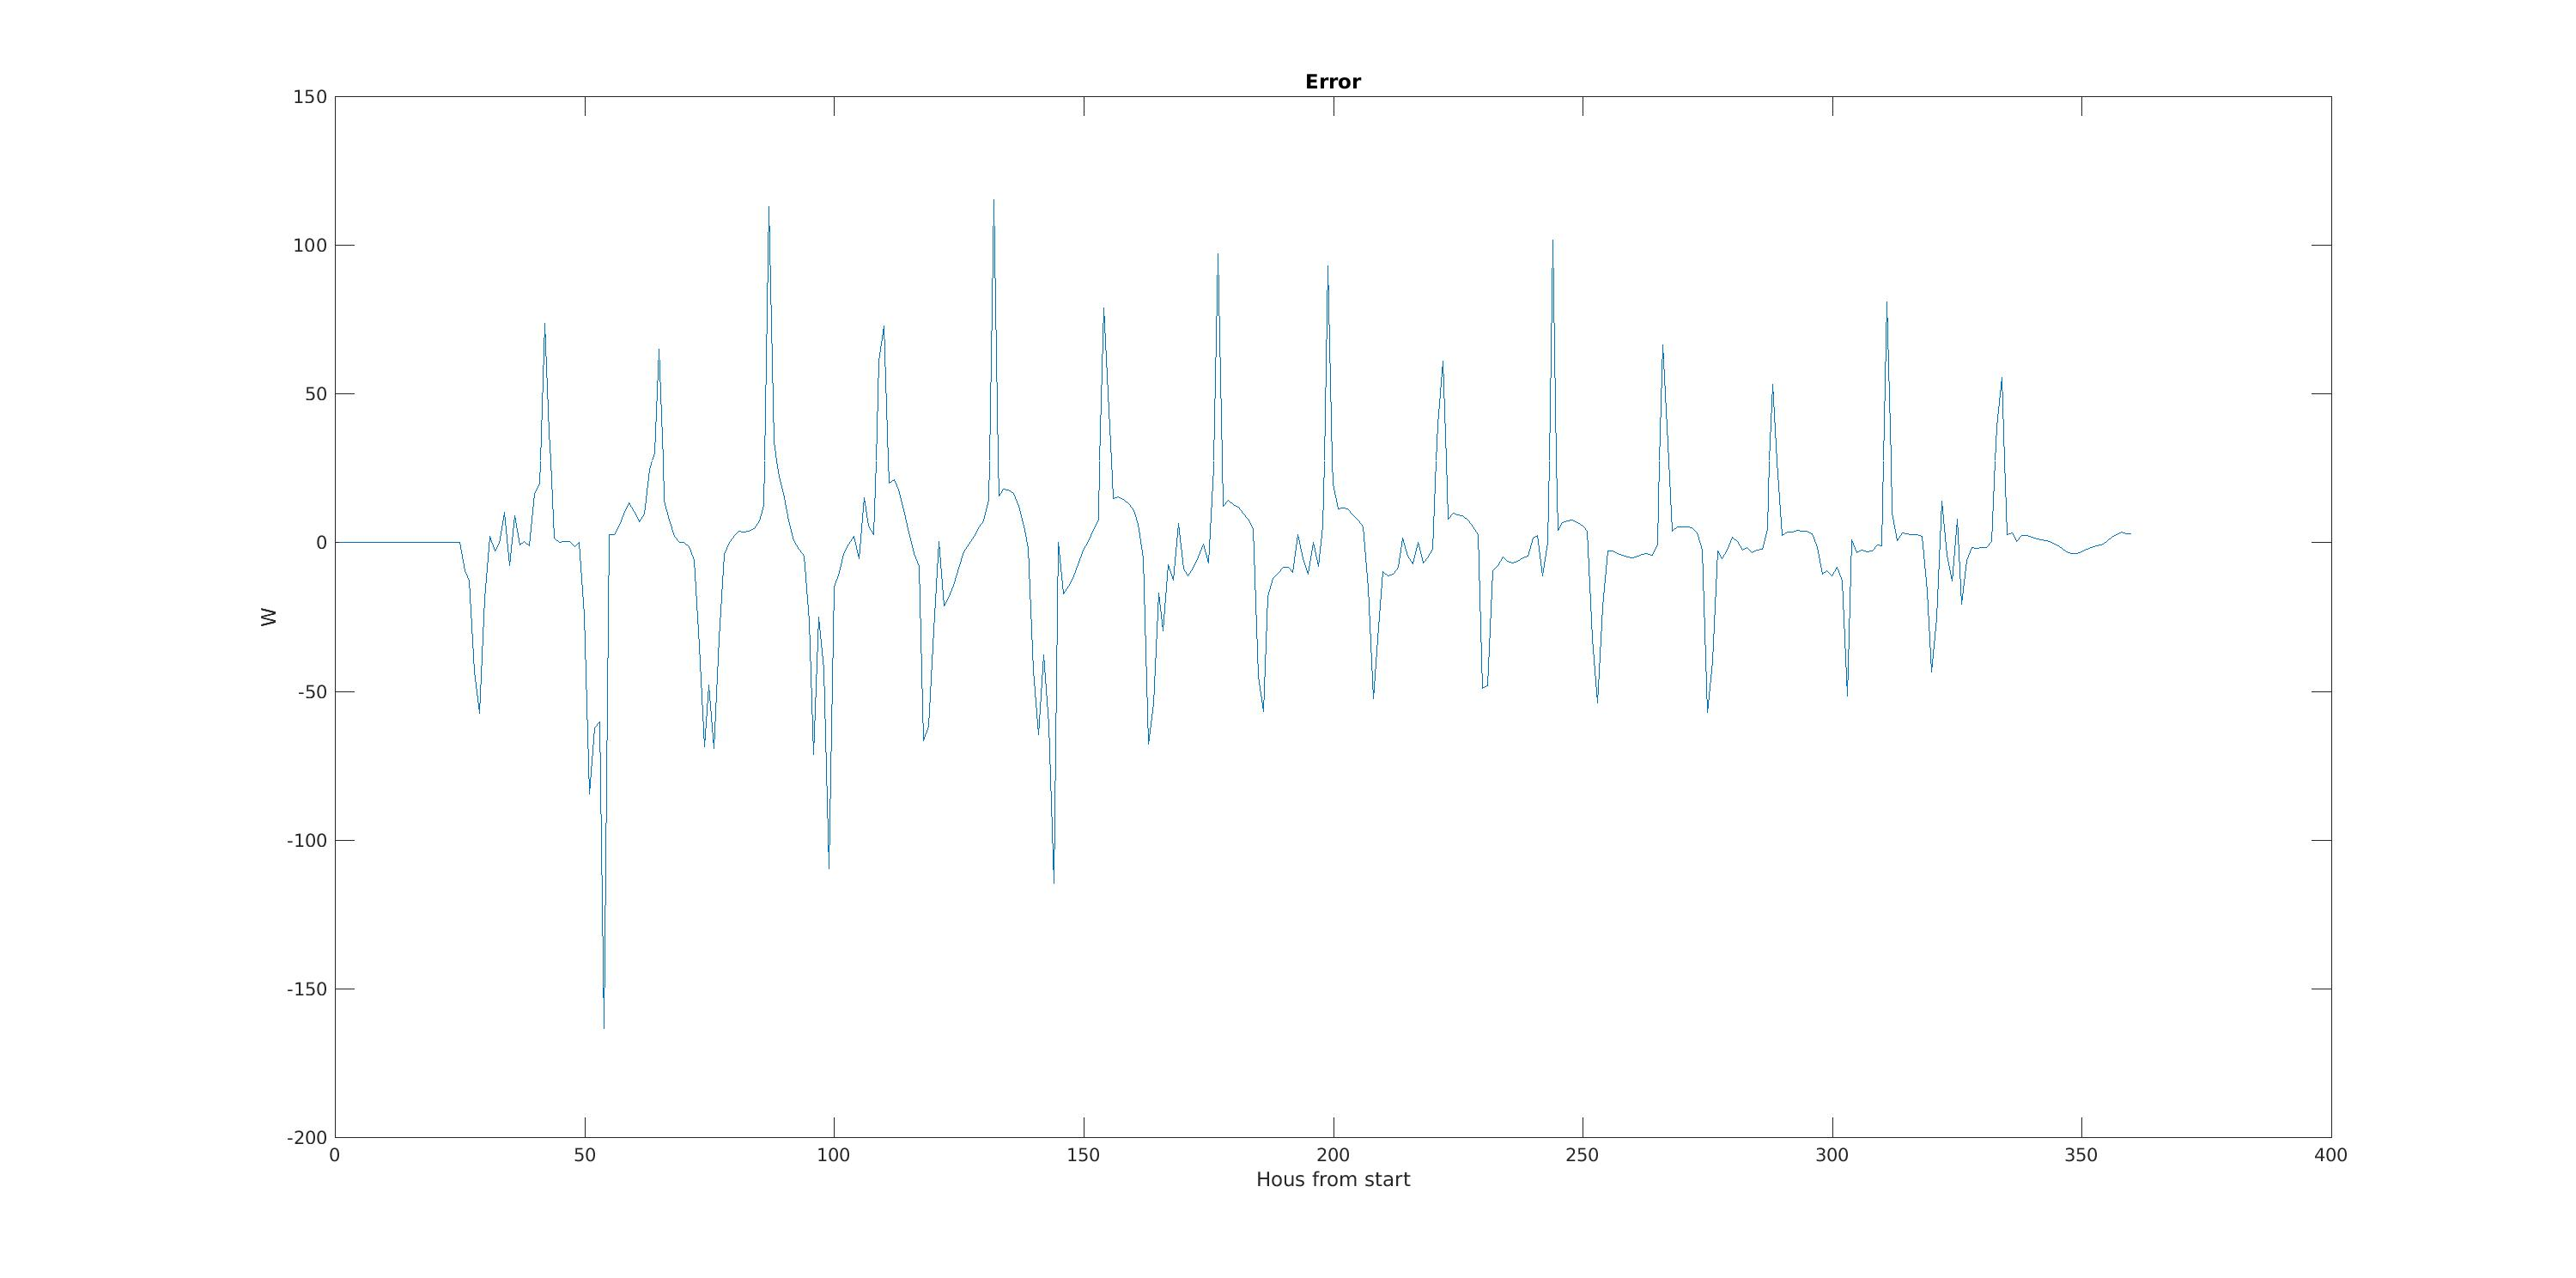
\includegraphics[width=\textwidth]{WCMA-PDR_error.jpg}
    \caption{WCMA with PDR Prediction error}
    \label{fig:wcmapdr_error}
\end{figure}


\subsubsection{Red neuronal artificial} 
\label{ssub:nn}

El resultado de la red neuronal es especialmente bueno si consideramos valores estables, pero el tiempo de procesado y aprendizaje (El cual deberá ser continuo)

\begin{figure}[h]
    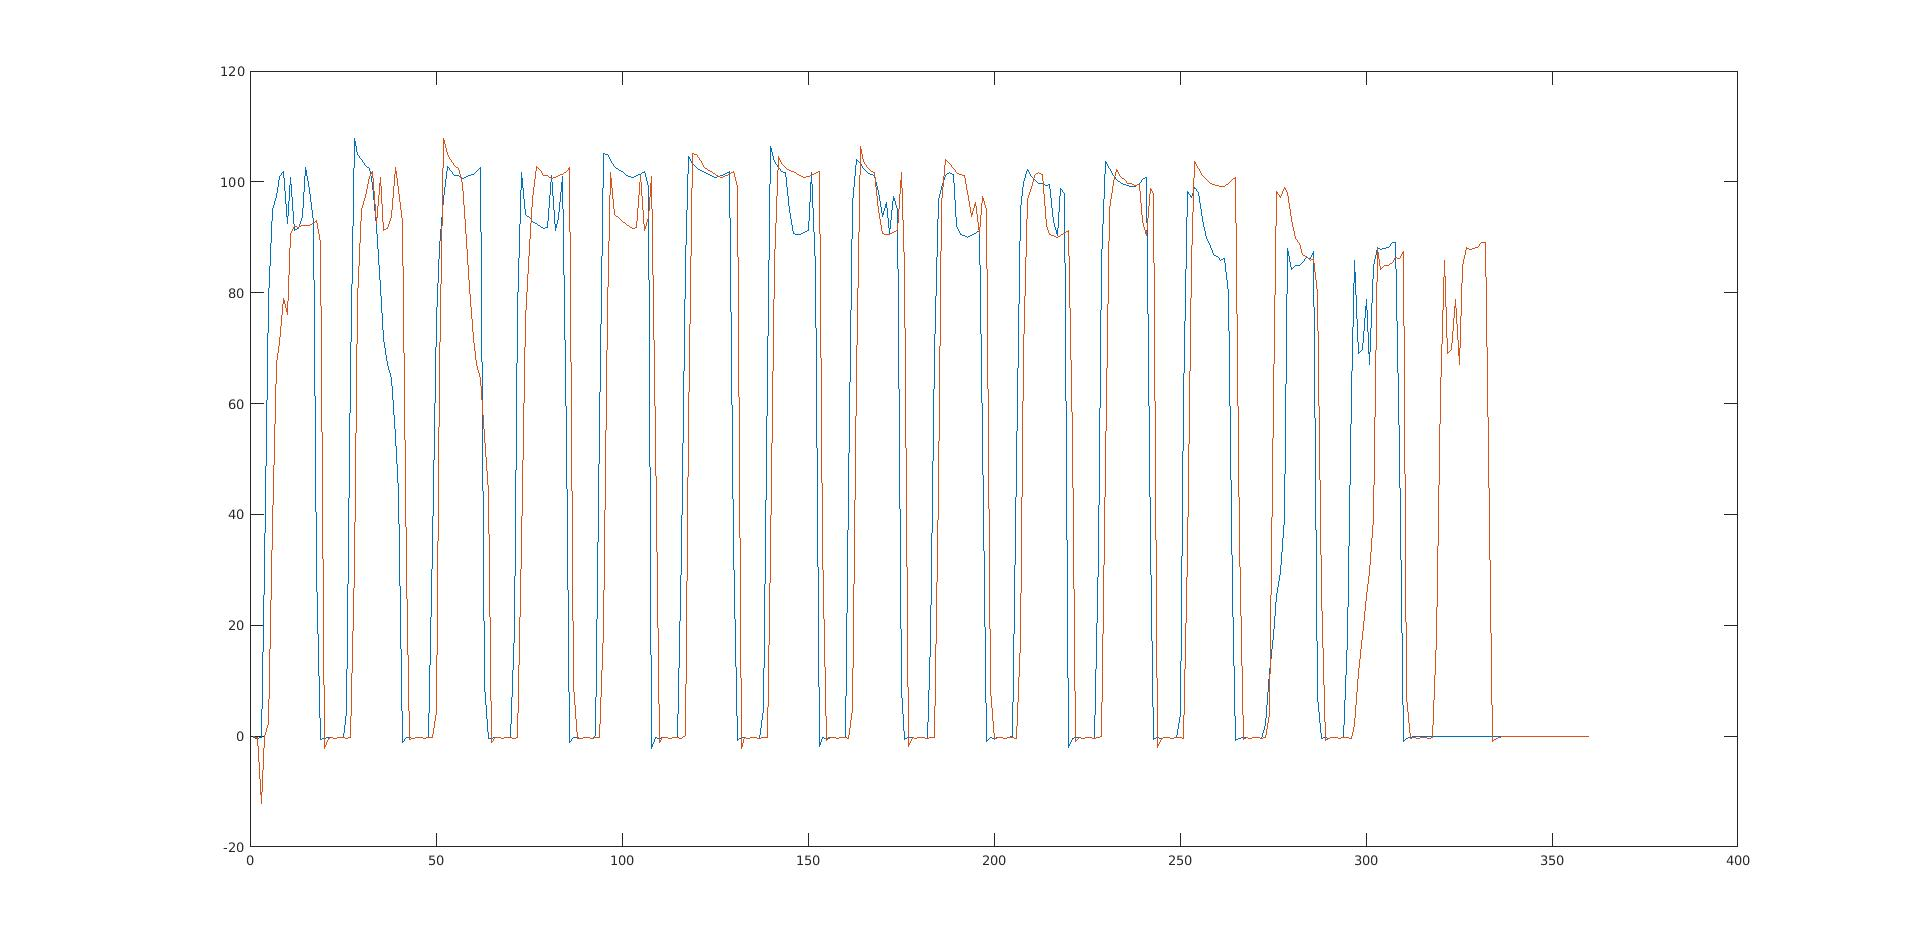
\includegraphics[width=\textwidth]{nn.jpg}
    \caption{neural network Prediction accurancy}
    \label{fig:nn_comp}
\end{figure}

\begin{figure}[h]
    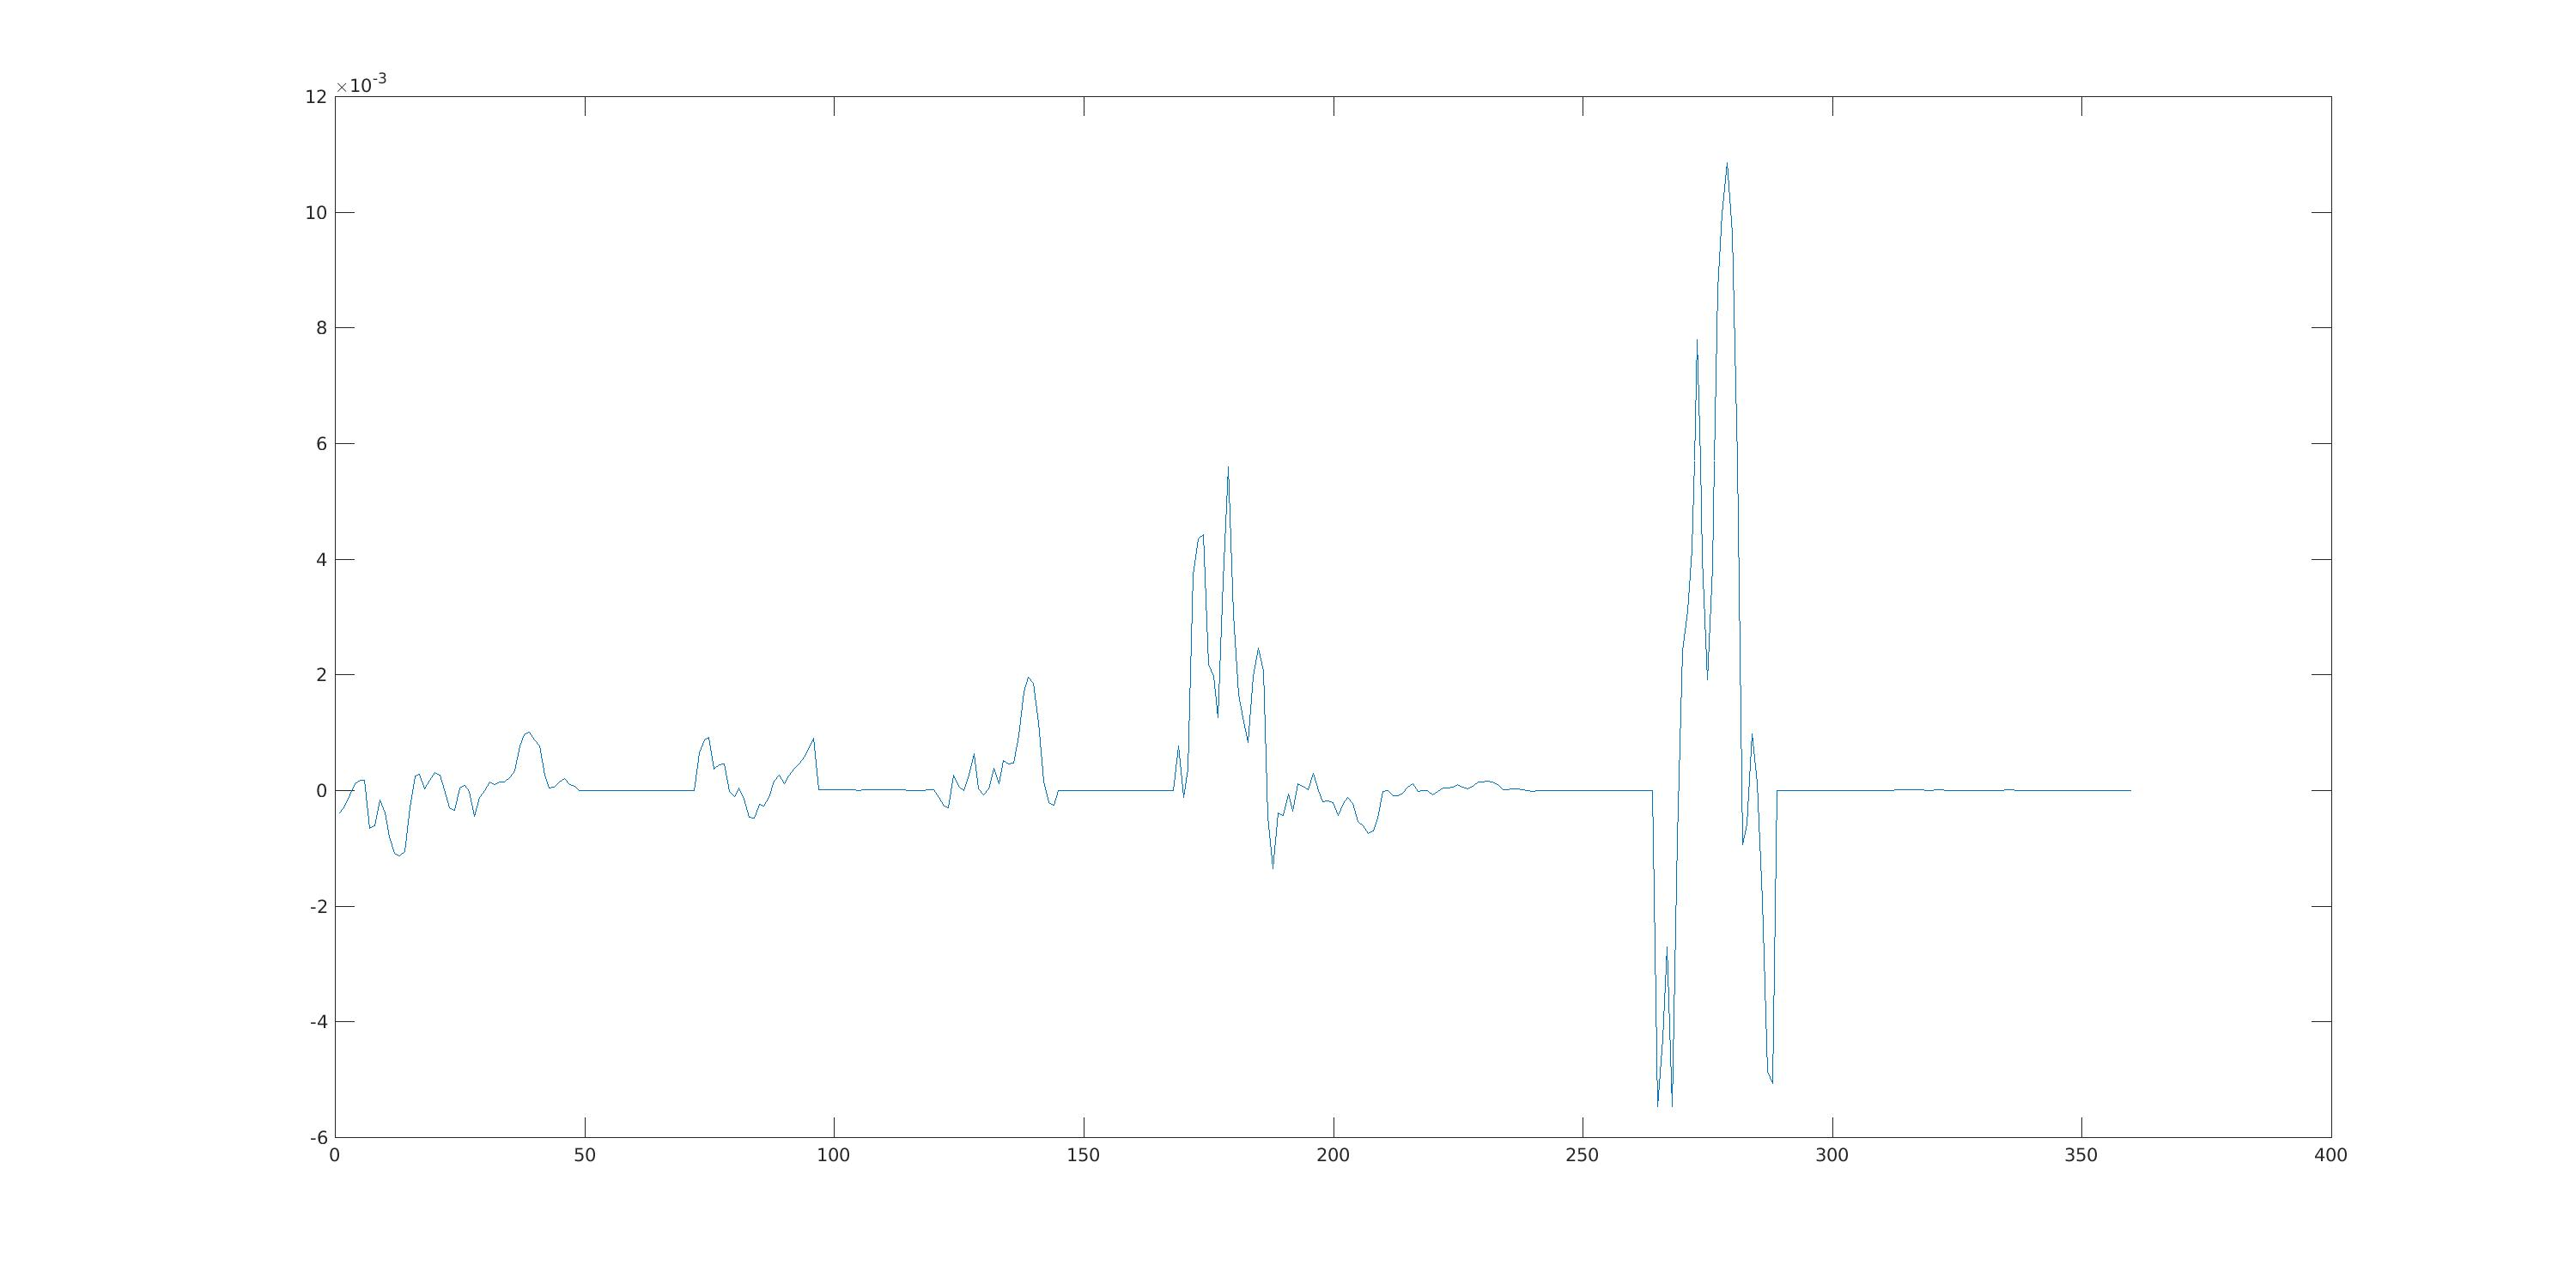
\includegraphics[width=\textwidth]{nn_error.jpg}
    \caption{neural network Prediction error}
    \label{fig:nn_error}
\end{figure}

